%%%%%%%%%%%%%%%%%%%%%%%%%%%%%%%%%%%%%%%%%
% Masters/Doctoral Thesis 
% LaTeX Template
% Version 2.5 (27/8/17)
%
% This template was downloaded from:
% http://www.LaTeXTemplates.com
%
% Version 2.x major modifications by:
% Vel (vel@latextemplates.com)
%
% This template is based on a template by:
% Steve Gunn (http://users.ecs.soton.ac.uk/srg/softwaretools/document/templates/)
% Sunil Patel (http://www.sunilpatel.co.uk/thesis-template/)
%
% Template license:
% CC BY-NC-SA 3.0 (http://creativecommons.org/licenses/by-nc-sa/3.0/)
%
%%%%%%%%%%%%%%%%%%%%%%%%%%%%%%%%%%%%%%%%%

%----------------------------------------------------------------------------------------
%	PACKAGES AND OTHER DOCUMENT CONFIGURATIONS
%----------------------------------------------------------------------------------------


\RequirePackage{snapshot}
\makeatletter
\def\snap@providesfile#1[#2]{%
  \wlog{File: #1 #2}%
  \if\expandafter\snap@graphic@test\expanded{#2}@@\@nil
    \snap@record@graphic#1\relax #2 (type ??)\@nil
  \else
    \expandafter\xdef\csname ver@#1\endcsname{#2}%
  \fi
  \endgroup
}
\makeatother

% SED command for extracting filenames of figures from dependency file
% sed -e '/Figures/!d' -e 's/  \*{file}   {//' -e 's/}{[0\/.v ]*}//' main.dep

\documentclass[
11pt, % The default document font size, options: 10pt, 11pt, 12pt
%oneside, % Two side (alternating margins) for binding by default, uncomment to switch to one side
english, % ngerman for German
singlespacing, % Single line spacing, alternatives: onehalfspacing or doublespacing
%draft, % Uncomment to enable draft mode (no pictures, no links, overfull hboxes indicated)
%nolistspacing, % If the document is onehalfspacing or doublespacing, uncomment this to set spacing in lists to single
%liststotoc, % Uncomment to add the list of figures/tables/etc to the table of contents
%toctotoc, % Uncomment to add the main table of contents to the table of contents
%parskip, % Uncomment to add space between paragraphs
%nohyperref, % Uncomment to not load the hyperref package
headsepline, % Uncomment to get a line under the header
%chapterinoneline, % Uncomment to place the chapter title next to the number on one line
%consistentlayout, % Uncomment to change the layout of the declaration, abstract and acknowledgements pages to match the default layout
]{MastersDoctoralThesis} % The class file specifying the document structure

\usepackage[utf8]{inputenc} % Required for inputting international characters
\usepackage[T1]{fontenc} % Output font encoding for international characters


\usepackage{mathpazo} % Use the Palatino font by default

\usepackage[style=authoryear, backend=biber, url=false]{biblatex} % Use the bibtex backend with the authoryear citation style (which resembles APA)

\addbibresource{main.bib} % The filename of the bibliography

% Set up hyperref for creating a non-default PDF starting page . This must be done before \usepackage, because that sets defaults that cannot be overwritten.
\usepackage{zref-abspage,zref-user} 
\makeatletter
\AtBeginDocument{%
  \zref@refused{chap:pdfstartpage}%
  \hypersetup{%
    pdfstartpage=\zref@extractdefault{chap:pdfstartpage}{abspage}{1}%
  }%
}
\makeatother


% Packages added by Niel:
\usepackage{hyphenat}
\usepackage{xspace}
\usepackage{hyperref}
\usepackage{bookmark}
\usepackage[]{todo}
\usepackage{eurosym} 
\usepackage{textcomp}
\usepackage[modulo]{lineno}
\usepackage{quotchap}
	\newcommand{\quotewidth}{80mm}
\usepackage{caption}
\usepackage{chemfig}
\usepackage{zref-abspage,zref-user}
\usepackage{refcheck}
\usepackage{tabulary}
%\usepackage{stampinclude}

% Command to generate list of files used in logfile
%\listfiles

% Not added by Niel, but needs to be after lineno
\usepackage[autostyle=true]{csquotes} % Required to generate language-dependent quotes in the bibliography

\linenumbers


% New definitions:
\newcommand\nox{\texorpdfstring{NO\textsubscript{x}}{NOx}\xspace}
\def\dotsign{\xleaders\hbox to .2em{\d{}}\hfill\d{}}
\newcommand{\oneD}{\textsuperscript{1}D\xspace}
\newcommand{\twoD}{\textsuperscript{2}D\xspace}

%----------------------------------------------------------------------------------------
%	MARGIN SETTINGS
%----------------------------------------------------------------------------------------

\geometry{
	paper=a4paper, % Change to letterpaper for US letter
	inner=2.5cm, % Inner margin
	outer=3.8cm, % Outer margin
	bindingoffset=.5cm, % Binding offset
	top=1.5cm, % Top margin
	bottom=1.5cm, % Bottom margin
 	%showframe, % Uncomment to show how the type block is set on the page
}

%----------------------------------------------------------------------------------------
%	THESIS INFORMATION
%----------------------------------------------------------------------------------------

\thesistitle{Fast temperature programmed gas chromatography coupled to supercritical fluid chromatography (SFC×GC)} % Your thesis title, this is used in the title and abstract, print it elsewhere with \ttitle
\supervisor{Prof. ER \textsc{Rohwer}} % Your supervisor's name, this is used in the title page, print it elsewhere with \supname
\examiner{} % Your examiner's name, this is not currently used anywhere in the template, print it elsewhere with \examname
\degree{Doctor of Philosophy} % Your degree name, this is used in the title page and abstract, print it elsewhere with \degreename
\author{Daniel \textsc{Malan}} % Your name, this is used in the title page and abstract, print it elsewhere with \authorname
\addresses{} % Your address, this is not currently used anywhere in the template, print it elsewhere with \addressname

\subject{Chemistry} % Your subject area, this is not currently used anywhere in the template, print it elsewhere with \subjectname
\keywords{} % Keywords for your thesis, this is not currently used anywhere in the template, print it elsewhere with \keywordnames
\university{University of Pretoria} % Your university's name and URL, this is used in the title page and abstract, print it elsewhere with \univname
\department{Department of Chemistry} % Your department's name and URL, this is used in the title page and abstract, print it elsewhere with \deptname
\group{Research Group Name} % Your research group's name and URL, this is used in the title page, print it elsewhere with \groupname
\faculty{Natural and Agricultural Sciences} % Your faculty's name and URL, this is used in the title page and abstract, print it elsewhere with \facname

\AtBeginDocument{
\hypersetup{pdftitle=\ttitle} % Set the PDF's title to your title
\hypersetup{pdfauthor=\authorname} % Set the PDF's author to your name
\hypersetup{pdfkeywords=\keywordnames} % Set the PDF's keywords to your keywords

}

\begin{document}

% Added to avoid error reported by pdfTeX
\pdfsuppresswarningpagegroup=1
 
\frontmatter % Use roman page numbering style (i, ii, iii, iv...) for the pre-content pages

\pagestyle{plain} % Default to the plain heading style until the thesis style is called for the body content

%----------------------------------------------------------------------------------------
%	TITLE PAGE
%----------------------------------------------------------------------------------------

\begin{titlepage}
\begin{center}

\vspace*{.06\textheight}
{\scshape\LARGE \univname\par}\vspace{1.5cm} % University name
\textsc{\Large Doctoral Thesis}\\[0.5cm] % Thesis type

\HRule \\[0.4cm] % Horizontal line
{\huge \bfseries \ttitle\par}\vspace{0.4cm} % Thesis title
\HRule \\[1.5cm] % Horizontal line

by \\
 
% \begin{minipage}[t]{\textwidth}
\Large
%\label{\href{http://www.johnsmith.com}}{\authorname} % Author name - remove the \href bracket to remove the link
\vspace{1em}
\textbf{\authorname}
\vspace{1em}

% \end{minipage}

Submitted in partial fulfilment of the requirements for the degree \\

% \begin{minipage}[t]{\textwidth}
\Large
%\label{\href{http://www.johnsmith.com}}{\authorname} % Author name - remove the \href bracket to remove the link
\vspace{1em}
\textbf{\degreename}
\vspace{1em}

% \end{minipage}


%\begin{minipage}[t]{0.4\textwidth}
%\begin{flushright} \large
%\emph{Supervisor:} \\
%\label{\href{http://www.jamessmith.com}}{\supname} % Supervisor name - remove the \href bracket to remove the link  
%{\supname}
%\end{flushright}
%\end{minipage}\\[3cm]
 
%\vfill

%\large \textit{A thesis submitted in fulfillment of the requirements\\ for the degree of \degreename}\\[0.3cm] % University requirement text
%\textit{in the}\\[0.4cm]
%\groupname\\\deptname\\[2cm] % Research group name and department name
In the Faculty of Natural \& Agricultural Sciences\\ University of Pretoria \\ Pretoria \\ 
 
\vfill

{\large 29 November 2019}\\[4cm] % Date
%{\large \today}\\[4cm] % Date
%\includegraphics{Logo} % University/department logo - uncomment to place it
 
\vfill
\end{center}
\end{titlepage}

%----------------------------------------------------------------------------------------
%	DECLARATION PAGE
%----------------------------------------------------------------------------------------

\begin{declaration}
\addchaptertocentry{\authorshipname} % Add the declaration to the table of contents

\noindent I, \authorname, declare that the thesis, which I hereby submit for the
degree PhD (Chemistry) at the University of Pretoria, is my own work and has not
previously been submitted by for a degree at this or any other tertiary
institution.

\vspace{2em} 
 
\makebox[.5\linewidth][l]{SIGNATURE: \dotsign\smallskip}\\

\makebox[.5\linewidth][l]{DATE: \dotsign\smallskip}\\
 
%\noindent SIGNATURE: 
%\rule[0.5em]{25em}{0.5pt} % This prints a line for the signature

%\noindent DATE:
%\rule[0.5em]{25em}{0.5pt} % This prints a line to write the date

\end{declaration}

\begin{ethicsdeclaration}
\addchaptertocentry{\ethicsname}

The author, whose name appears on the title page of this thesis, has obtained, for the research described in this work,
the applicable research ethics approval.

The author declares that he/she has observed the ethical standards required in terms of the University of Pretoria’s
Code of ethics for researchers and the Policy guidelines for responsible research.


\end{ethicsdeclaration}
\cleardoublepage

%----------------------------------------------------------------------------------------
%	QUOTATION PAGE
%----------------------------------------------------------------------------------------

\vspace*{0.2\textheight}

\noindent\enquote{\itshape Learning is a peculiar compound of memory, imagination, scientific habit,
accurate observation, all concentrated, through a prolonged period, on the
analysis of the remains of literature. The result of this sustained mental
endeavour is not a book, but a man.}\bigbreak

\hfill Mark Pattison

%----------------------------------------------------------------------------------------
%	ABSTRACT PAGE
%----------------------------------------------------------------------------------------

\begin{abstract}
\addchaptertocentry{\abstractname} % Add the abstract to the table of contents

The Thesis Abstract is written here (and usually kept to just this page). The
page is kept centered vertically so can expand into the blank space above the
title too\ldots


\end{abstract}

%----------------------------------------------------------------------------------------
%	ACKNOWLEDGEMENTS
%----------------------------------------------------------------------------------------

\begin{acknowledgements}
\addchaptertocentry{\acknowledgementname} % Add the acknowledgements to the table of contents

I gratefully acknowledge my supervisor, Prof Egmont Rohwer, who had the faith in
me to invite me to take on the project, and the patience to wait for me to
respond and the patience to wait for me to finish. 

Dok Fanie (Dr SJ van der Walt) my predecessor, showed me how to be bold in the
lab. He was the giant on whose shoulders I stand.

I acknowledge my fellow students,
\begin{itemize} 
  
\item Kobie Smit lent a kind ear to the laments, and helped me feel less alone.

\item Marc Bouwer, whose youthful energy proved to be highly contagious, spent
hours in front of the whiteboard with me, helping to clarify thoughts and
understanding basic science.

\item Elize Smit, who set me such a good example of academic performance. Thank
goodness I didn't try to follow it.
 
\item Linda Pretorius, whose PhD challenges made me grateful for the simplicity
of my project.

\item Nadine Broodryk for all the conversations.

\item My office mates, in no particular order: Sifiso Nsibande, Madelien
Wooding, Kedibone Mashale, Portia Makhubela, Chiedza Munyeza, Amanda Mahlangu,
Genna-Leigh Geldenhuis, Margaux Lim-a-Tock, Leandri van der Wat, Basil Mujanja,
Olu Adegoke, Hanieh Montaseri.

\end{itemize}

My father, Danie Malan, spent time and energy and time on instrument making. My
mother, Retha Malan, ensured that I was fed and dressed. 

Of course the project would not have been possible without the assistance from
the technical team at the University of Pretoria:

\begin{itemize}
\item Our instrument maker, Nico van Vuuren, whose excellent work inspired me to
create designs worthy of that quality of work.

\item My thanks to David Masemula, who maintained the supply of consumables.

\item Yvette Naudé is a most kind and helpful lab manager.

\item Naomi Steenkamp is the most quietly effective financial administrator known to
man. Through her services purchasing supplies supplies was a painless experience.

\item Annetjie Kok and Ria Swart were kindest administrators.

\item Antoinette of the Centre for Microscopy and Microanalysis at the
University of Pretoria provided invaluable aid in collecting the SEM images.

\item Dr Erna Gerryts, Faculty Academic Advisor, was my thesis writing manager.
This is a unique role, and she was uniquely qualified to fill it. The existence of this thesis

\end{itemize}

Our commercial suppliers also need acknowledgement. Beyers at Chemetrix, who
spent extra effort in keeping instrumentation running. For Agilent, who supplied
us with an excellent used intrument at a nominal cost. Restek provided us with a
set of HPLC columns at no cost. Reynard Heymans from FLIR recorded thermal
videos of the coaxial heater in action without asking for money. Neil Frame from
D.C. Wort supplied me with free samples and offered valuable advice.

Mathilda Mosterd of Precision Oils Laboratories Pty Ltd provided me with
prepared samples and their fatty acid profiles, which afforded valuable
comparisons.

My mental health team kept me sane. Johan Erasmus, whose professional
psychological help first guided me through clinical depression, and then was
crucial in getting me unstuck. Maria Ramaahlo at the Disability Unit was the
first person to offer concrete help with ADHD. Dr GP Grobler, my competent
psychiatrist, always offered interesting conversations, despite his limited
time. Dr Zuleikha Ahmed of Student Support treated me with the utmost kindness,
even when I was extremely angry. And of course the innumerable staff members of
Virgin Active Health Clubs always made visiting their gym a very pleasant
experience.

Sasol Fuel supported the laboratory through funding.

The financial assistance of the South African National Energy Research Institute
towards this research is hereby acknowledged. Opinions expressed and conclusions
arrived at, are those of the author and are not necessarily to be attributed to
SANERI.

Sunil Patel, in true hacker spirit, made the \LaTeX template this document is
based on freely available.


\end{acknowledgements}

%----------------------------------------------------------------------------------------
%	PREFACE
%----------------------------------------------------------------------------------------

\begin{preface}
\addchaptertocentry{\prefacename}

People learn from other people. In the academic environment, students formally
learn from professors and from trusted authors of academic writing. Less
formally, students also learn from other students, and what other students
wrote, including dissertations and theses.

In the South African academic environment, students often lack a wide base of
knowledge: they survive a secondary education system that has the bare minimum
of resources, and then enter a highly-focused tertiary degree programme. When
they graduate, they are well-trained and are knowledgeable in a narrow technical
field. They rarely have had the time to obtain knowledge extending beyond their
formal academic programme.

This thesis was therefore written with the following audience in mind: A young
South African who has successfully passed through the South African school
system, has just obtained an Honours degree in chemistry at the University of
Pretoria, and is now embarking on a postgraduate degree. The thesis starts by
putting the scientific work strongly in context of history, society, and
technology before elaborating on the theoretical and technical work and finally
presenting the results obtained.

\end{preface}

%----------------------------------------------------------------------------------------
%	LIST OF CONTENTS/FIGURES/TABLES PAGES
%----------------------------------------------------------------------------------------

\tableofcontents % Prints the main table of contents

\listoffigures % Prints the list of figures

\listoftables % Prints the list of tables

%----------------------------------------------------------------------------------------
%	ABBREVIATIONS
%----------------------------------------------------------------------------------------

\begin{abbreviations}{ll} % Include a list of abbreviations (a table of two columns)


\textbf{CCGT} & Combined Cycle Gas Turbine \\
\textbf{DIO} &  Digital Input/Output\\
\textbf{EOF} &  Efficiency-Optimized Flow\\
\textbf{EOV} &  Efficiency-Optimized Velocity\\
\textbf{EPC} &  Electronic Pneumatic Control\\
\textbf{FAME} &  Fatty Acid Methyl Ester\\
\textbf{FID} &  Flame Ionization Detector\\
\textbf{GC} & Gas Chromatography\\
\textbf{GC×GC} &  Comprehensively coupled Gas Chromatography\\
\textbf{GHG} & Greenhouse Gases \\
\textbf{HPLC} & High-Performance Liquid Chromatography\\
\textbf{IPCC} & Intergovernmental Panel on Climate Change\\
\textbf{LCA} & Life Cycle Analysis \\
\textbf{LC×GC} &  Comprehensively coupled (Liquid Chromatography × Gas Chromatography)\\
\textbf{MV} &  Manipulated Variable\\
\textbf{\nox} &  Nitrogen Oxides (NO, NO$_2$, NO$_3$ and N$_2$O, and N$_2$O$_5$)\\
\textbf{PID} &  Proportional Integral Derivative\\
\textbf{PLOT} & Porous Layer Open Tubular\\
\textbf{PV} &  Process Variable\\
\textbf{PWM} &  Pulse-Width Modulation \\
\textbf{SFC} & Supercritical Fluid Chromatography \\
\textbf{SFC×GC} &  Comprehensively coupled (Supercritical Fluid × Gas Chromatography)\\
\textbf{SIM} &  Single Ion Monitoring \\
\textbf{SOF} &  Speed-Optimized Flow\\
\textbf{SOV} &  Speed-Optimized Velocity\\
\textbf{SPE} & Solid Phase Extraction\\
\textbf{SV} &  Set Value \\
\textbf{TLC} & Thin-Layer Chromatography \\
\textbf{UNFCCC} & United Nations Framework Convention on Climate Change \\



\end{abbreviations}

%----------------------------------------------------------------------------------------
%	PHYSICAL CONSTANTS/OTHER DEFINITIONS
%----------------------------------------------------------------------------------------


%\begin{constants}{lr@{${}={}$}l} % The list of physical constants is a three column table

% The \SI{}{} command is provided by the siunitx package, see its documentation for instructions on how to use it

%Constant Name & $Symbol$ & $Constant Value$ with units\\


%\end{constants}
%----------------------------------------------------------------------------------------
%	SYMBOLS
%----------------------------------------------------------------------------------------

\begin{symbols}{lll} % Include a list of Symbols (a three column table)

\textbf{Symbol} & \textbf{Name} & \textbf{Unit}\\

\( a \) & selectivity & dimensionless  \\
\( k' \) & retention factor & dimensionless\\
\( P_M \) & modulation period & \si{\second} \\
\oneD & first dimension & \\
\twoD & second dimension & \\
\( t_r \) & retention time & \si{second}\\
\( \eta \) & energy efficiency & dimensionless\\
\( \eta_{C} \) & Carnot energy efficiency & dimensionless\\
\( \eta_{CM} \) & Chambadal-Novikov energy efficiency & dimensionless\\
\( V \) & electrical potential difference &  \si{\volt} \\
\( I \) & electrical current & \si{\ampere}\\
\( P \) & power & \si{\watt}\\
\( p_o \) & outlet pressure & \si{\pascal}\\
\( \Delta p \) &  pressure difference & \si{\pascal}\\
\( T \) & temperature & \si{kelvin} \\
\( N \) &  number of plates & dimensionless \\
\( E \) & chromatographic efficiency & dimensionless \\

%$P$ & power & \si{\watt} (\si{\joule\per\second}) \\
%Symbol & Name & Unit \\

%\addlinespace % Gap to separate the Roman symbols from the Greek

%$\omega$ & angular frequency & \si{\radian} \\

\end{symbols}

%----------------------------------------------------------------------------------------
%	DEDICATION
%----------------------------------------------------------------------------------------

\dedicatory{Dedicated to the memory of Dr. Barbara Lotze} 

%----------------------------------------------------------------------------------------
%	THESIS CONTENT - CHAPTERS
%----------------------------------------------------------------------------------------

\mainmatter % Begin numeric (1,2,3...) page numbering

\pagestyle{thesis} % Return the page headers back to the "thesis" style


%----------------------------------------------------------------------------------------

% Define some commands to keep the formatting separated from the content 
\newcommand{\keyword}[1]{\textbf{#1}}
\newcommand{\tabhead}[1]{\textbf{#1}}
\newcommand{\code}[1]{\texttt{#1}}
\newcommand{\file}[1]{\texttt{\bfseries#1}}
\newcommand{\option}[1]{\texttt{\itshape#1}}

%----------------------------------------------------------------------------------------

% Include the chapters of the thesis as separate files from the Chapters folder
% Uncomment the lines as you write the chapters

%\setcounter{chapter}{-1}% Chapter Template

\chapter{Thesis Organization} % Main chapter title

\label{Chapter0} % Change X to a consecutive number; for referencing this chapter elsewhere, use \ref{ChapterX}

The topic of this thesis is the development of a comprehensively coupled
(supercritical fluid × gas) chromatograph (SFC×GC) and its application to the
analysis of biodiesel. The purpose of this chapter is to clearly and succinctly
explain the content of this thesis and to act as a guide to the reader.

The thesis is divided into five parts, each containing up to three chapters.
Figure~\ref{fig:ThesisOrganization} contains a diagrammatic representation of
its structure.

\begin{description}
 
\item{Part \ref{sec:Part1}}{ provides a scientific background framed in terms of
the molecular basis of sustainability and addresses the question ``Why was the
research done?'' It discusses the climate crisis and constructs an argument 
based on thermodynamics that biodiesel is likely to find a place in its solution
(Chapter~\ref{Chapter1}), explains the use of carbon dioxide as a ''green
chemical'' in analytical chemistry and chromatography and introduces the concept
of SFC×GC (Chapter~\ref{Chapter2}), and describes the chemical properties of a
commercially-viable biodiesel and explains the use of chromatography in the
quality control of biodiesel (Chapter~\ref{Chapter3}).}

\item{Part \ref{sec:Part2}}{ covers the apparatus used and addresses the
question ``How was the research done?'' It describes the development of the
instrumentation used for supercritical fluid chromatography (SFC)
(Chapter~\ref{Chapter4}), explains the need and introduces the theory of fast
temperature-programmed GC and then describes the development of a gas
chromatograph that can perform four temperature\hyp{}programmed
(\SIrange{-20}{350}{\celsius}) runs per minute (Chapter~\ref{Chapter5}).}

\item{Part \ref{sec:Part3}}{ contains the experimental results, and addresses
the question ``What was found?'' It demonstrates the chemical separation of the
main components of biodiesel (Chapter~\ref{Chapter6}), the separation of
biodiesel/petrodiesel blends (Chapter~\ref{Chapter7}), and the promise of using
volatile co-solvents with carbon dioxide in SFC×GC-FID (Chapter~\ref{Chapter8}).}

\item{Part \ref{sec:Part4}}{ contains the concluding Chapter~\ref{Chapter9},
which addresses the question ``What progress was made?'' It reprises the main
argument of the thesis, summarizes the contributions of the research, discusses
its shortcomings, and suggests directions for future research.}

\item{Part \ref{sec:Part5}}{ contains appendices with technical information and the bibliography.} 

\end{description}

\begin{figure}[htbp]
\centering
\includegraphics[width=\textwidth]{Figures/ThesisOrganization.pdf}
\decoRule
\caption[Thesis Organization]{A diagrammatic guide to the structure of this thesis.}
\label{fig:ThesisOrganization}
\end{figure}

\begin{savequote}[60mm]
C\textsubscript{n}H\textsubscript{2n+2} + O\textsubscript{2} $\rightarrow$ CO\textsubscript{2}+ H\textsubscript{2}O + \SI{45}{\kilo\joule\per\gram}\\
CO\textsubscript{2} + H\textsubscript{2}O + h$\nu$ $\rightarrow$ C\textsubscript{6}H\textsubscript{22}O\textsubscript{2} 
\qauthor{Hydrocarbons give heat and sunshine makes sugar}
\end{savequote}

\chapter{Introduction: Climate, fuel, and biodiesel} % Main chapter title

\label{Chapter1} % Change X to a consecutive number; for referencing this chapter elsewhere, use \ref{ChapterX}

% ----------------------------------------------------------------------------------------
% SECTION 1
% ----------------------------------------------------------------------------------------

\section{Energy, fuel and the atmosphere}

Industrialized societies depend on reliable sources of energy. For the purpose
of this discussion, the main types of energy can be counted as electricity and
fuels, although they are interconvertible. Fuels for industrialized societies
are predominantly found as underground mineral deposits, from where they are
extracted by mining or drilling. They are found as solids, liquids and gases,
which the energy industry refers to as \textit{coal}, \textit{crude oil}, and
\textit{natural gas}. Because these fuels are of biological origin, deposited
during previous geological eras, and then metamorphosed and preserved by
geological processes, these fuels are commonly referred to as `fossil fuels'.

The large-scale exploitation of fossil fuels started in the middle of the 18th
century, when the plentiful coal from the coalfields of Great Britain drove a
development that is is known to history as the Industrial Revolution. This
development is closely associated with steam engines \autocite{Rosen2012}. The
use of crude oil started in the middle of the 19th century, and is associated
with the development of the automobile \autocite[p. 42]{Watts2005}. The use of
natural gas started in the middle of the 20th century and is associated with the
introduction of gas-fired central heating in for homes in cold climates
\autocite{Hanmer2017} Fossil fuels also serve as feedstock to the chemical
industry, but that topic lies outside the scope of this discussion.

There is no doubt that the use of fossil fuels as an energy source greatly
improved the human lot. The mechanization of agriculture and the easy
distribution of food by motorized transport have eliminated famine as a natural
disaster \autocite{Angelis2007}. The distribution of medical supplies by
motorized transport and the rapid deployment of medical personnel have limited
the impact and spread of epidemics \autocite{Ministere2018}. Heating and cooling
of buildings have increased the habitable zone on earth. Artificial light has
increased the hours available for mental activity, in particular extending the
reach of entertainment, art and education.

However, in the context of chemistry, the uncontrolled use of fuels has at
least two major problems.

The first problem with fossil fuel is that it is finite. There is only a certain
amount of fossil fuel on earth. If all of it is extracted it will no longer be a
reliable source of energy, and the existence of industrialized societies and the
complex civilizations that depend on them will be in jeopardy. It is tempting to
think that civilizations would have the foresight to prepare for such an
eventuality, but the historical record shows that societies can collapse when at
the height of their powers \autocite{Diamond2006}.

The second problem with fuels is that they produce pollution wherever they are
produced, processed, transported and used. Pollution is injurious to the health
and well-being of individuals, societies and nature. If pollution is serious
enough, it not only degrades society and the environment, but also negates the
benefits brought by the application of energy: modern hospitals are
energy-intensive, but if they are filled with victims of pollution there is no
nett benefit.

The first approach to pollution from fuels has been to ignore it. Pictures
from the early industrial revolution shows English towns coated with soot and
choked with smoke \autocite{Flick1980}, and rivers became toxic
sewers \autocite{Halliday2001}.

The development of public health, social responsibility \autocite{Szreter2003}
and an embryonic environmental movement \autocite{Williams1965} lead to
political pressure for the implementation of pollution controls, which governments
gradually introduced and increased in strictness.

The first generation of pollution control offered essentially two options:
concentrate or dilute.

%\footnote{Abatement is also an option, but if economic
%competition is strong then abatement is a natural outcome of the drive towards
%efficiency: every atom of carbon in the fuel not turned into carbon dioxide
%represents lost revenue, hence organic pollutants tend to be minized by economic
%forces. Those of us who saw the fall of the Berlin wall remember the revelation
%of the extreme pollution emitted by Communist industry. The same might not be
%true for other pollutants.}

I will illu\-strate these two options using a typical South Afri\-can coal-fired
pow\-er sta\-tion. In such a power station coal is burned to produce heat, which
converts liquid water into high-pressure steam. The steam is allowed to expand
through a turbine, which converts the energy in the steam into rotary motion,
which is used to turn an alternator that produces an electric current by
rotating a set of electrical conductors in a magnetic field. The furnaces of
such a power station produce a flow of waste. This waste is an \textit{aerosol}:
finely divided solids suspended in a mixture of gases. 

The solid part is typically separated from the gas-phase part by filter bags and
electrostatic precipitators: the collected material is known as \textit{fly
ash}. The gas-phase part might be sent through scrubbers to remove some of the
gas-phase pollutants, capturing it in a solid form. The solid part of the power
station's furnace waste has now been concentrated. It is transported to a
storage site, where it is stored indefinitely. It goes without saying that
concentrated pollutants should be encapsulated during storage in some way,
otherwise they just become more sources of pollution.

The gas-phase part of the pollutant is handled by diluting it. The outlet for
the gas-phase stream of waste is through a tall stack, which ends high above
ground level\footnote{The chimneys of those sooty Victorian towns were not there
to disperse the smoke, but to create a `draft', a flow of air created by the
buoyancy of hot air. The better the draft, the more efficient the fire.}. At
this altitude the wind is strong and steady, which rapidly carries the gases and
remaining aerosols away and disperses them.

The dilution of pollutants might seem like an abdication of responsibility, but
it is an reasonable response to pollution. At low enough concentrations
pollutants that enter the biosphere are broken down by sunlight and microbes
which render it harmless. This makes dilution a reasonable first attempt at
controlling pollution.

The devil is, of course, in the detail. For example, mercury that find its way
into the environment is eventually converted by microbes to methyl mercury,
which concentrates in aquatic animals. All rivers in the continental USA are now
polluted by airborne mercury that originate from coal-fired power stations
\autocite{Wentz2014}. Some persistent organic pollutants, which also concentrate
in the food chain, originate in fuel combustion. So while dilution was a
reasonable first attempt at controlling pollution, it it certainly not the final
answer.

The majority of fuels provide their energy as heat, which can be converted into
useful work. This heat is obtained by combining the chemical compounds found in
the fuel with atmospheric oxygen to form compounds with lower internal energy. The
maximum amount of work that can be extracted from a given fuel can be estimated
by examining the Gibbs free energy equation:

\begin{equation}
	\Delta G = \Delta H - T \Delta S
\label{eq:Gibbs}
\end{equation}

For a given compound fuel compound, $\Delta H$ is determined by the difference
in enthalpy of formation of the product waste compounds and the enthalpy of
formation of the reactant fuel compounds. Since the reactant fuel compounds are
given, $\Delta H$ is maximized by having product compounds with very low
enthalpies of formations.

To maximize $\Delta S$, the products should be as disordered as possible. This
implies that \emph{gas-phase} products composed of \emph{small molecules} will
yield more work.

The temperature $T$ should also be as high as possible.

Because the industrial machinery in economically competitive, capital-intensive
industries are highly efficient, the maximum amount of energy is extracted from
their fuels for the lowest cost. Following Gibbs, the major compounds left over
after extracting the energy from a fuel should have very low enthalpies of
formation and be in the gas phase at the temperature of the process. 

Because all fuels contain carbon as a major component, the extraction of energy
yields compounds containing carbon. Most fuels also contain hydrogen. Reacting
these fuels with the oxygen in air to extract maximal work will therefore
yield water (H$_2$O) and carbon dioxide (CO$_2$). 

(Of course the argument is not that Victorian engineers designed steam engines
using the Gibbs energy equation, but the variation-selection process
\autocite[Chapter 8]{Vincenti1990} by which engineering improvements accrue would
inevitably drive the development of heat engines fuelled by fossil fuels to emit
large quantities of carbon dioxide gas.)

Water is of course not a pollutant at all, and carbon dioxide is only toxic at
very high concentrations, and therefore, for most of the industrial era, carbon
dioxide was easily dealt with by by diluting it in the atmosphere, where it is
also naturally present at low levels. To the extent that carbon dioxide was
considered a pollutant it was assumed that it would be absorbed by the
biosphere.

Photosynthesis, the process by which green plants capture the energy from
sunlight to live and grow, does indeed remove carbon dioxide from the
atmosphere, and an elementary model of the carbon cycle that assumes stability
would seem to indicate that excess carbon dioxide in the atmosphere would be
captured by photosynthesis and sequestered, leaving the carbon dioxide
concentration in the atmosphere stable. Of course this model contains
testable assumptions, which scientists could, and did, test.

The most famous of these tests is probably the ``Keeling Curve''
\autocite{Harris2010}. This is a continuous record of measurements of
concentration of atmospheric carbon dioxide in the pristine air of the Pacific
Ocean. This record starts in 1958 and shows that the carbon dioxide
concentration of the atmosphere is increasing.

Paleoclimatologists have studied the hypothesis that the carbon dioxide
concentration is stable over time. Not only have they found that the carbon
dioxide concentration is \emph{not} stable, they have also determined that the
pre-industrial concentration of atmospheric carbon dioxide was lower than it was
in 1958 \autocite{Petit1999}.

So it is clear that the carbon dioxide concentration in the atmosphere is rising
because of the biosphere is not absorbing all the carbon dioxide produced by the
combustion of fossil fuels. 

The projected concentration of carbon dioxide in the atmosphere is, however,
still not at or even near toxic levels, which might make the continued dilution
of carbon dioxide in the atmosphere seem a viable disposal method.

Emitted gases, however, do not only have chemical properties and biological
impacts, they also have physical properties. Of concern for the current
discussion is carbon dioxide's absorbance of electromagnetic radiation, in
particular the radiation arriving from the sun, and the radiation from the
earth's surface out to space, both which must pass through the atmosphere. A
molecule can absorb parts of this radiation by having its electrons excited, or
by changing its vibration. Carbon dioxide is electronically very stable, and
therefore absorbs only extreme ultraviolet radiation, just like the major gases
in the atmosphere, molecular nitrogen and molecular oxygen. However it poorly
absorbs near ultraviolet and visible light, in which is it also similar to the
major gases. Because there is a dipole moment between the carbon atom and the
oxygen atoms of carbon dioxide, it has vibrational modes which can absorb
radiation in the infrared region of of the electromagnetic spectrum. Oxygen and
nitrogen do not have dipole moments, and therefore do not absorb infrared
radiation strongly. This means that carbon dioxide will absorb infrared
radiation in the atmosphere much more strongly than the major gases. The energy
from the absorbed infrared radiation is of course turned into vibration, a form
of kinetic energy, and this kinetic energy is randomly further distributed among
the gases of in the atmosphere, appearing as an increase in temperature as the
energy distribution moves towards equilibrium.

The most cursory understanding of the absorption of infrared radiation in the
atmosphere by carbon dioxide therefore seems to say that an increase in the
concentration of carbon dioxide in the atmosphere would lead to a higher average
temperature in the atmosphere. This increase in temperature was first estimated
by Svante Arrhenius in 1896 \autocite{Arrhenius1897}.

(The other major product of extracting energy from fuel is water. Its molecule
also has a dipole moment, and it also absorbs infrared radiation strongly.
However, its intermolecular properties sets an upper limit to its concentration:
at high enough concentrations it will either condense into water or crystallize
into ice and precipitate from the atmosphere to end up as surface water.)

Further research has only confirmed that industrial processes extracting energy
from fuel is increasing the amount of carbon dioxide in the atmosphere by
gigatons every year, and that this increase in concentration is leading to
higher temperatures in the atmosphere. It had also become increasingly certain
that this increase in temperature is inevitable and significant: it will change
earth's climate\footnote{The atmosphere is in contact with the hydrosphere, and
the two exchange carbon dioxide. The carbon dioxide diluted in the atmosphere is
therefore also diluted in the oceans. This leads to \textit{ocean
acidification}, a gigaton problem in it's own right, but one that falls outside
the scope of this discussion.}. This projected increase in temperature and the
accompanying change in global climate is bound to have impact on societies
within the lifetime of people alive today, and a larger impact on future
generations. Some of these projected changes are incompatible with the
maintenance of the complex civilizations that are supported by industrialized
societies \autocite{IPCC2014}.

Scientists do not inhabit ivory towers, and their research is funded by public
money in the expectation that the resulting science will benefit their
societies. As the understanding of carbon pollution grew, it became obvious to
scientists that industrialized societies could not just continue diluting
gigatons of carbon dioxide in the atmosphere, and they alerted policymakers. The
iconic moment of this development was the testimony of Dr James E. Hansen, at
the time director of NASA's Goddard Institute of Space Studies, before the
Senate of the US Congress in 1988 \autocite{Shabecoff1988}. In the same year the
scientists of the world came together and established the Intergovernmental
Panel on Climate Change (IPCC) to create a coherent body of knowledge to inform
decision-making. The IPCC has so far produced a series of five Assessment
Reports, which assesses the science of climate change, its impacts, and ways to
mitigate it \autocite{Allen2014}.

(Carbon dioxide is not the only greenhouse gas and the IPCC reports consider
each in detail, but because the other gases are not produced in significant
quantities by fuels and the energy industry they fall outside the scope of this
discussion.)

Industrialized societies currently depend on energy from fossil fuels. Huge
investments have been made in infrastructure, large numbers of people find
employment in this industry, and available alternative sources of energy are not
nearly sufficient. The health and well-being of the greater part of the world's
population depend on it. But the future health and well-being of those same
societies also depend on ending that dependence. It would be in the best
interest of industrialized societies to create plans to reduce the dependence on
energy from fossil fuels and exploit alternative energy sources.

But industrialized societies are also in economical competition with each other.
This means that any society that spends resources on risky, expensive
alternative sources of energy risks falling into a competitive disadvantage, and
there is a surfeit of short-sighted politicians who will take advantage of
this risk to create fear and so prevent planning for and investment in
changes in energy production and use\footnote{The impact of political corruption
is not negligible, but I will abstain from commenting on it.}.

Fortunately there are enough leaders who have vision, and based on the
recommendations of the IPCC the governments of the world have come together to
create the UNFCCC. The United Nations Framework Convention On Climate Change is
an international agreement that structures the response of nations to limit
their emissions of greenhouse gases. Two international treaties have been agreed
to so far: the Kyoto Protocol in 1997 \autocite{Kyoto1997} and the Paris
Agreement in 2015 \autocite{Paris2015}.

These agreements attempt to reduce the amount of carbon dioxide released into
the atmosphere by dividing the cost of reducing emissions fairly. While the
Kyoto Protocol invoked a complex carbon credit trading scheme, in the Paris
Agreement nations pledge to reduce emissions of carbon dioxide into the
atmosphere, and each is free to do so in a way that suits them best.

The Republic of South Africa is a signatory to the Paris Agreement, and
therefore the country is legally bound to limit and reduce its emissions of
carbon dioxide and other greenhouse gases. The country has so far promised to
stop increasing emissions between 2020 and 2025 \autocite{INDC2016}.

% ----------------------------------------------------------------------------------------
% SECTION 2 --------------------------------

\section{Carbon footprints and carbon neutrality}

Ending the emission of carbon dioxide by industrialized societies is an exercise
in balancing effort with consequences. Every reduction in carbon dioxide
emissions must necessarily have an effect on the economy, and conversely, every
change in economic activity will have an effect on carbon dioxide emissions.

A rational, discerning society in searching for ways to carbon dioxide
emissions will therefore attempt to change their economy in such a way that the
emission of carbon dioxide is limited or reduced. But in most societies there
are many ways to reduce carbon dioxide emissions, and decisions have to be
made on which ones to implement. Such decisions must be based on sound information,
and one way to generate that information is a discipline called \textit{life
cycle analysis} (LCA). 

Life cycle analysis can yield rigorously-calculated data and comparisons, but it
is a very general method. For analyses that are very similar and differ only in
context, it is possible to develop simplified, standardized life-cycle analysis tools.

One such tool is the \textit{carbon footprint}. Every economic activity in an
industrialized society generates emissions of greenhouse gases.
These emissions might  be far removed from the activity in space and time. A
most obvious example of this is the use of electricity: At the moment I'm using
a computer to compose this paragraph and electric light illuminates the desk I'm
working on here in my office in Pretoria. The electricity that powers the
computer and the lamps are generated hundreds of kilometres from here, most of
it on the Mpumalanga Highveld, in coal-fired power stations which emits carbon
dioxide in the process. So my activity is far removed from the associated
emissions \textbf{in space}. But even before the coal was burned, the machines that mined
it and transported it to the power station emitted carbon dioxide, so my
activity is also removed from the emissions \textbf{in time}. The sum of all these
emissions connected with my activity constitute the carbon footprint of my
activity.

Although carbon footprinting is conceptually straightforward, it is analytically
rigorous and computationally complex. But there are standard protocols
\autocite{WRI2004} that can be followed, so that carbon footprints from
different activities and different organizations are transparent and comparable.

Once an organization's activities have been footprinted, the organization can
examine its operations and look at ways to change activities that will reduce
that footprint.

If my university, for example, decides to install photovoltaic panels on the roof
of my building, and use the electricity to illuminate my office, the activity
will now most likely have a reduced carbon footprint, because photovoltaic
electricity usually has a lower carbon footprint than coal-derived electricity.

To prevent a climate disaster, at some point industrialized societies will have
to change all their activities until they no longer emit any greenhouse gases.
Such activities will have carbon footprints of zero, and will be known as
`carbon neutral activities'. There are also activities that are nett removers of
carbon from the atmosphere, which would be `carbon negative'.

In truth, in industrialized societies there are very few carbon neutral
activities. Even if I'm just sitting quietly in a pristine nature reserve, the
food I am digesting and metabolizing have a positive carbon footprint: carbon
was emitted to fix nitrogen from the air, which was used as fertilizer to help
grow the food I ate, and is now in the proteins of my body. The very calcium and
phosphorus in my bones were sourced from mines that were powered by fossil
fuels. 

\section{Internal combustion engines.}

Carbon footprinting exercises quickly show that a major source for emissions is
transport. Most transport in industrialized societies is powered by
internal\hyp{}combustion engines. They are called `internal\hyp{}combustion' engines
because the chemical transformation that extracts the energy from the fuel is
internal to the engine. This is in contrast to the power station steam turbines
mentioned earlier, where the extraction of the chemical energy from the fuel
happens outside of the engine. The engine is the device that produces the
mechanical energy. These engines are usually powered by liquid fuels derived
from crude oil, although some designs run on gas, and of course in South Africa
Sasol and PetroSA supply us with liquid fuels derived from coal and natural gas.

This discussion will use the term \textit{noxious pollution} to describe
pollution that is directly harmful to humans and \textit{carbon pollution} to
describe pollution that leads to industrial climate disruption.

The simplest way to reduce an activity's carbon footprint is to use the fuel
that drives that activity more efficiently. Fortunately market forces are
aligned with this, because more efficient use of a fuel also reduces running
costs. Discussing engine designs therefore almost always invokes
\textit{efficiency}. Efficiency of an engine is calculated by taking the ratio
output power:input power. The greek letter $\eta$ is used as a symbol for
efficiency:

\begin{equation}
\eta = \frac{P_{out}}{P_{in}}
\label{eqn:efficiency}
\end{equation}

Conservation of energy dictates that the output power cannot be more than the
input power, and therefore \(\eta \leq 1\). The power is `lost' to two factors:
firstly entropy, as dictated by the Second Law of Thermodynamics, and secondly
losses, such as friction.

\subsection{Scaling and efficiency} \label{par:scaling}

The efficiency of engines scales disproportionately with its linear dimensions,
by which is meant that the larger an engine is, the more efficient it is. There
are three factors that improve efficiency in larger engines \autocite{Brown2017}:

\begin{enumerate}

\item Longer residence time: In larger engines, the reacting fuel spends more
time in the engine. This gives reactions more time to reach equilibrium, and
hence more energy can be extracted.

\item Smaller surface area to volume ratio: The volume of an engine increases
with the cube of its linear dimension, but the surface area increases with the
square of its linear dimensions. This means that larger engines have a smaller
surface-to-volume ratio than smaller engines. Since losses take place at the
surface, the loss per unit volume is therefore larger for smaller engines than
it would be for larger engines of the same type. If the losses in larger engines
are comparatively smaller, we can expect larger engines to be more
efficient than smaller ones. 
  
\item Larger Reynolds number: The Reynolds number is a number that predicts the
onset of turbulent flow, and is calculated from the viscosity, velocity and a
characteristic linear dimension.  The higher the Reynolds number, the higher the
likelihood of turbulent flow. Turbulent flow promotes mixing, which leads to
improved combustion and hence higher efficiency. The larger the engine, the
larger the characteristic linear dimension, and therefore the higher the
likelihood of turbulent flow.

\end{enumerate}

From the viewpoint of reducing carbon pollution, one should therefore aim to use
a few large engines rather than a multitude of small engines.

\subsection{Engine design and thermodynamic cycles.} \label{par:efficiency}

The final design of a successful internal combustion engine is determined by the
variation-selection process described by Vincenti \autocite{Vincenti1990}. Such
a design sufficiently satisfies a wide range of requirements. These requirements
might be explicitly expressed in documentation, or they may be implied, or they
may be practical. These requirements would include, but are not limited to,
capital cost, running cost, maintenance cost, noise, sound, ease of maintenance, power
output, emissions, surface finish, weight, mounting method, size, supply chain
capability, shape, colour, fuel availability, operating temperature, altitude
tolerance and torque.

From designers' attempts to fulfil these requirements arise the myriad of
different engine designs, delivering anything from milliwatts to megawatts of
power to anything from model aircraft to oil tankers. It is the good fortune of
researchers who study engine efficiency that there are only a few conceptual
systems that explain how the internal combustion engines convert the chemical
energy of the fuel into mechanical work.

The principles on which the different engines operate are named `cycles',
because the way they convert heat into work can be describe in terms of a series
of events that are repeated endlessly. The concept of a cycle is
further entrenched because it is customary to explain the thermodynamic
processes involved using at \textit{pV} diagram, showing the changes of state of
the working fluid during engine operation.

Theoretical thermodynamic cycles are useful because they can predict the
performance of heat engines, allowing for comparison. In particular, it allows
for comparison with theoretical maxima. The maximum efficiency of a heat engine
is delivered by an engine running on the Carnot cycle. This describes a
hypothetical engine that uses only reversible processes to extract useful work
from the temperature difference between two reservoirs of heat. It has been
shown that the Carnot cycle offers the maximum possible heat extraction, and
that the maximum efficiency (\(\eta_{C}\)) is determined solely by the temperature
difference between the hot (\(T_h\)) and the cold (\(T_c\)) reservoirs.

\begin{equation}
	\eta_{C} = 1 - \frac{T_c}{T_h}
\label{eqn:Carnot}
\end{equation}

The Carnot cycle, however, can only deliver an infinitesimal amount of work,
because the heat transfer must be reversible, and therefore infinitesimal. A
more realistic maximum efficiency is given by the Chambadal-Novikov efficiency
(\(\eta_{CN}\)) \autocite{Hoffmann2008}:

\begin{equation}
	\eta_{CN} = 1 - \sqrt{\frac{T_c}{T_h}}
\label{eqn:Chambadal-Novikov}
\end{equation}

This theoretical efficiency takes into account the irreversible processes that
are inevitable in engines delivering finite amounts of power.

Barring revolutionary new discoveries and inventions, there will be only three
thermodynamic cycles and their corresponding internal combustion engines on the
market, as we enter the low-carbon era.

\subsubsection{Otto engine and Otto cycle}

The oldest of the internal combustion engines is the Otto engine. It is named
after Nikolaus Otto, who developed the first working engine of this kind in 1876
\autocite[Chapter 9]{Cummins1989}. In South Africa these engines are usually
called `petrol engines`.

In the Otto engine, a homogeneous mixture of atmospheric air and vaporized fuel
is compressed. This mixture is then ignited by an electric spark. The energy
released by the chemical reaction between the oxygen in the air and the fuel
vapour causes the temperature of the compressed air to rise, and consequently
the pressure. If this, now hot, gas is allowed to expand in an expandable
vessel, the motion of the vessel can be captured to perform useful work. Once
the useful work is extracted, the vessel can be collapsed again to expel the
exhausted air, and re-filled with a compressed air/fuel vapour mixture. This
completes the cycle. The expandable vessel is usually in the form of a cylinder
and piston, with the piston connected to a crank that drives a shaft that
transfers the work from the engine to the machine being powered.

\begin{figure}
\centering
\includegraphics[width=\textwidth]{Figures/otto-cycle}
\decoRule

\caption[The Otto cycle]{The pV diagram of the thermodynamic Otto cycle. The
isochoric heat addition step (BC) corresponds to the burning of the homogeneous
air-fuel mixture. Work is extracted from the engine during the adiabatic
expansion CD \autocite{Wolfram|Alpha2019Otto}. }

\label{fig:otto-cycle}
\end{figure}

(These legs of the cycle are only loosely related to the `strokes' of a
four-stroke engine, and should not be confused for them.)

The theoretical efficiency of the Otto Cycle is given by 

\begin{equation}
	\eta = 1 - (\frac{1}{r^{\gamma-1}})
\label{eqn:otto-efficiency}
\end{equation}

where \(r\) is the \textit{compression ratio}, \( \frac{V_1}{V_2} \), and
\(\gamma\) is the heat capacity ratio, which can considered a constant for the
purposes of this discussion \autocite{Wolfram|Alpha2019Otto}.

This means that the efficiency of an Otto engine can be improved by increasing
the degree of compression of the intake air before combustion. 

\subsubsection{Diesel Cycle}

In the Diesel engine, named after Rudolf Diesel who demonstrated the first
engine of this type in 1897 \autocite[Chapter 14]{Cummins1989}, air is
compressed, and then a finely divided solid or liquid fuel is injected into the
system. The fuel then reacts with the oxygen in the air. The energy released in
the reaction appears as a higher temperature in the gas, and --- following
Gay-Lussac's Law --- the pressure of the gas rises. If the gases expands in the
confines of a collapsible vessel, useful work can be extracted from expansion of
the vessel. Once the work has been extracted, the vessel can be collapsed again
to remove the now inert ('exhausted') gas and prepare for receiving the next
charge of air, completing the cycle.

The theoretical cycle used to analyse the performance of the Diesel Engine is
called the Diesel Cycle. (See figure \ref{fig:diesel-cycle})

\begin{figure}
	\centering
	\includegraphics[width=\textwidth]{Figures/diesel-cycle}
	\decoRule

	\caption[The Diesel cycle]{The pV diagram of the thermodynamic Diesel cycle. The
	isobaric process BC corresponds to the combustion of the finely divided fuel
	particles in air. Work is extracted from the engine both during this process and
	during the adiabatic process CD. \autocite{Wolfram|Alpha2019Diesel}}

	\label{fig:diesel-cycle}
\end{figure}

The Diesel cycle differs from the Otto cycle in the heat addition step. In the
Otto engine, the heat addition takes place when the homogeneous air/fuel mixture
combusts. This combustion takes place in a short space of time during which
the engine parts move only a negligible distance. Hence the pressure rises
rapidly. In the Diesel engine, the fuel is injected into a volume of compressed
air, where it combusts. (There is no separate ignition source: the temperature
of the adiabatically compressed air is higher than the fuel's ignition
temperature, so that the fuel ignites upon injection. While this is another
difference between the two engines, it is of second-order importance when
discussing thermodynamic cycles.) Because the combustion takes place at the
surface of fuel particles, the combustion rate is lower than the combustion rate
of the homogeneous mixture in the Otto cycle. Hence the rising temperature is
balanced by the motion of the engine, and the heat addition is essentially
isobaric.

The efficiency of the Diesel cycle is given by Equation \ref{eqn:diesel-efficiency}

\begin{equation}
	\eta = 1 - \frac{1}{r^{(\gamma - 1 )}}(\frac{\alpha^{\gamma}-1}{\gamma(\alpha-1)})
\label{eqn:diesel-efficiency}
\end{equation}
 
where \(\alpha\) is the \textit{cut-off ratio} and \(\gamma\) is the compression ratio.

The term \( \frac{\alpha^{\gamma}-1}{\gamma(\alpha-1)} \) is always larger
than \(1 \), and therefore, when we compare equation \ref{eqn:diesel-efficiency}
with equation \ref{eqn:otto-efficiency} it is clear that for a given
compression ratio the Diesel cycle is always less thermally efficient than the
Otto cycle. 

However, at high compression ratios Otto engines start suffering from
`knocking', when the homogenous air/fuel mixture detonates, instead of burning
smoothly. The shock waves from this detonation will damage the engine and lead
to faster wear. (The \textit{octane number} of a fuel indicates the compression
ratio it can accommodate.) Because Diesel engines do not suffer from this
problem, they can, and usually are, designed to operate at higher compression
ratios than Otto engines.  Otto engines normally operate with a compression
ration of up to 9:1, where as Diesel engines have compression ratios of up to
25:1. This makes Diesel engines significantly more efficient than Otto engines. 

\subsubsection{Gas turbines and the Brayton Cycle}

The third internal\hyp{}combustion engine important to industrialized society is
the \textit{gas turbine}. Gas turbines are used rarely in road transport, more
often in marine and stationary applications, but thousands take to the sky
every day, propelling aircraft \autocite{Morris2017} carrying billions of airline
passengers every year.

The first gas turbines were developed during wartime urgency to deliver pure jet
thrust for military aircraft, but this proved to be an inefficient use of the
available energy. Most modern turbine engines drive a shaft to extract
rotational work. This shaft might drive a bypass fan (as used in airliner engines), a
propeller (as used in smaller, low-speed aircraft), or a shaft which might drive
a helicopter rotor or an electrical generator.

In operation, a gas turbine compresses air with one or more compressor stages.
The compressed air passes through a combustion chamber, where fuel is added and
combusted. As the now hot gases expand they pass through one or more turbine
stages, which is connected to drive the compressor and the output shaft, which
extracts work from the system. After the gas has passed through the turbine it
returns to atmospheric pressure, optionally doing work on the engine in the form
of thrust.

The theoretical thermodynamic cycle that is customarily used to analyse the gas
turbine is called the Brayton cycle, named after George Brayton, who
successfully manufactured a reciprocating engine based on this cycle. (See
figure \ref{fig:brayton-cycle}) Such engines are no longer
manufactured \autocite[Chapter 10]{Cummins1989}.

\begin{figure}
	\centering
	\includegraphics[width=\textwidth]{Figures/brayton-cycle}
	\decoRule
	
	\caption[The Brayton cycle]{The pV diagram of the thermodynamic Brayton cycle.
	In the gas turbine the continuous combustion of the injected fuel and free
	expansion of the air through a turbine means that the heat addition (BC) is
	isobaric. Work is extracted during the adiabatic expansion process CD
	\autocite{Wolfram|Alpha2019Brayton}.}
	
	\label{fig:brayton-cycle}
\end{figure}

The efficiency of the Brayton cycle is given by equation
\ref{eqn:brayton-efficiency} 

\begin{equation}
	\eta = 1 - \frac{T_{1}}{T_{2}} = 1 - (\frac{ P_{1} }{ P_{2} })^{(\frac{\gamma-1}{\gamma})}
\label{eqn:brayton-efficiency}
\end{equation}

where \(\gamma\) is the compression ratio \autocite{Wolfram|Alpha2019Brayton}.

Because the fuel is continuously added to the compressed air and the combustion
takes place in a heterogeneous mixture, gas turbines do not suffer from
`knocking' and therefore there is no upper limit to the compression ratio. The
main figure determining the efficiency of the engine is the turbine inlet
temperature, (\textit{i.e.} the outlet temperature of the combustion chamber)
which reaches 1600 °C in modern engines.

\subsection{Noxious pollution from internal combustion engines. }

Carbon pollution is not the only pollution emitted by internal combustion
engines. There is also noxious pollution, which affects the societies in which
they are used. There are ways to reduce or eliminate such pollution, but the
implementation of such measures affect the efficiency of the engine. 

Noxious pollution from internal\hyp{}combustion engines come from different sourc\-es
and have different effects.

\subsubsection{Unburnt fuel}

The combustion reactions in internal\hyp{}combustion engines are very fast, but
they are never at equilibrium. This means that at the end of a cycle, the
exhaust gases expelled from the engine contains, besides the carbon dioxide,
also chemical intermediates and unreacted fuel molecules.

Unreacted fuel is a noxious pollutant, not only in its own right, but also,
during the decomposition process in the environment, chemical reactions induced
by sunlight produces ozone, a reactive oxygen species that leads to respiratory
problems in victims of pollution \autocite{Davidson1998}.

Some of the fuel-like pollutants from internal\hyp{}combustion engines are not
present in the fuel. These compounds are formed in a process that might be
called \textit{pyro-synthesis}. They are themselves more stable than the
compounds from which they originate, but not as stable as the combustion end
products, carbon dioxide and water. Because they are themselves quite stable,
they require high temperatures to combust, which might not be achieved before
they leave the engine as waste. Notable pollutants from this source are the
policyclic aromatic hydrocarbons (PAH) and, if trace amounts of chlorinated
substances are present in the fuel, dioxins

One of the products of pyro-synthesis is particles of soot. These particles are
agglomerations of nano-sized particles of pure, amorphous carbon. The
agglomerations might include adsorbed PAHs and acids. Soot particles are very
stable and only react at very high temperatures. Diesel engines in particular
have a reputation for producing soot \autocite{Mohankumar2017}.

The final pollutant that can be classed as originating from partially combusted
fuel is carbon monoxide. It forms readily when fuels are burned in oxygen-poor
environments. Modern, well-maintained engines is a relatively rare cause of
acute carbon monoxide poisoning \autocite{Reumuth2018}, but chronic exposure to
low levels of environmental carbon monoxide has harmful effects
\autocite{Wright2002}.

\subsubsection{Contaminants and additives.}

Crude oil and coal contains not only carbon and hydrogen, but also other
elements, most notably sulfur and nitrogen. Depending on the refining process,
these elements might find their way into fuels. Organic nitrogen and sulfur will
easily oxidize and form stable oxides, yielding energy. Once outside the engine,
however, the volatile oxides will dissolve in any water in the air, forming
acids. \autocite{Duncan2016}

Fuel manufacturers add additives to fuels for various reasons, such boosting
octane rating or preventing corrosion. The prime example of additives as a
source of noxious pollution was tetraethyllead, which was added to petrol as an
octane booster. The emitted lead compounds was shown to be a pollutant that lead
to neurological impairment in its victims, and its use was phased out
\autocite{Needleman2000}.

\subsubsection{Side-reactions}

Most internal combustion engines use atmospheric air as oxidant. This air is
21\% oxygen, and 78\% nitrogen. Although nitrogen is very stable and inert, at
high temperatures it can react with oxygen. These reactions produce the oxides
of nitrogen: NO, NO$_2$, NO$_3$ and N$_2$O, and N$_2$O$_5$. They are
collectively called \nox.

These oxides can participate in the cycle that causes the photochemical smog.
They will also dissolve in atmospheric water and form acids: this might happen
far from the point of emission, resulting in \textit{acid rain}. 

\subsection{Mitigating pollution from internal\hyp{}combustion engines.}
 
Pollution from internal combustion engines is a social ill, and most governments
have regulations in place to limit and reduce this pollution. Engine and fuel
manufacturers are working hard to reduce this pollution.

The noxious pollution from internal combustion engines can be reduced by various
improvements, but there are three complementary approaches: fuel formulation
\autocite{Gertler1999}, cleanup \autocite{Braun2018} and engine management
\autocite{Reif2015}.

\subsubsection{Fuel formulation}

Adding oxygenates improves the octane rating of fuel and reduces \nox formation. 

\subsubsection{Exhaust gas cleanup} \label{par:cleanup}

Exhaust gases from internal combustion engines can be ``cleaned'', and there are
basically two approaches. The first is catalytic conversion, in which the
exhaust gases that contain the pollutants are passed over a catalyst bed. The
catalyst (a proprietary formulation of platinum, palladium and/or rhodium),
adsorbs the uncombusted volatile organic carbons, and oxidizes them. It
simultaneously catalytically decomposes \nox to molecular nitrogen and oxygen.

Secondly, filter systems can be used to remove particulate matter. 

\subsubsection{Engine management} \label{par:engine-management}

As described above, the main source of noxious pollution from
internal\hyp{}combustion engines is uncompleted or undesired chemical reactions,
and is not fundamental to the operation of the engine. By carefully managing the
engine system, noxious pollution can be reduced. 

The oldest engine management technology is the oxygen or `lambda' sensor, which
measures the oxygen in the exhaust gases. Such a sensor, coupled to an
engine-management computer, allows the me\-ter\-ing of the exact amount of fuel
need\-ed for op\-ti\-mum combustion \autocite{Frauhammer2014}.

A newer technology is known as exhaust gas recirculation. This mixes the intake
air of the engine with exhaust gases, effectively diluting the oxygen. This
reduces peak temperatures, and thereby \nox formation.

In \textit{stratified charge} engines the distribution of fuel in the volume of
intake air is controlled by selective fuel injection. Carefully injecting the
fuel at the right place at the right time can allow for higher compression
ratios without inducing pinging. \textit{Lean-burn} engines are Otto engines
that use use extremely high air:fuel ratios.

Electronic engine management systems result in much more efficient and
less-polluting engines than non-managed `mechanical' engines, but because
engines for automotive applications endure such a wide range of operating
conditions, they can at best achieve a compromise between power, efficiency and
emissions. It was this unsatisfactory compromise that lead to the Volkswagen
emissions scandal: manufacturers chose to cheat on emissions test rather than
admit to the relatively poor performance of a managed engine optimized for low
emissions \autocite{Mansouri2016}.

\subsubsection{Efficiency implications}

Attempts to mitigate noxious pollution from internal\hyp{}combustion engines
mostly lead to losses in efficiency. For example:

\begin{itemize}

\item Exhaust gas flow through catalytic converters and filters consume energy.
  
\item The engines cannot approach their theoretical maximum efficiencies,
because reducing \nox emissions is handled by limiting maximum combustion
temperatures.

\item \nox reduction catalysts require the presence of hydrocarbons,
\textit{i.e.} incomplete reactions, which implies that not all energy is
extracted from the fuel.

\item Every treatment system added to the engine adds weight to the vehicle, which
reduces payload and hence the total efficiency.

\end{itemize}

Before carbon dioxide pollution was a concern, it made sense to accept lower
efficiencies as a necessary cost of reducing noxious pollution, but in a
low-carbon future we cannot just keep on trading less noxious pollution for more
carbon dioxide production.

\subsection{Avoiding pollution from internal\hyp{}combustion engines} \label{par:carbon-neutral}

The efficiency and cleanness of internal\hyp{}combustion engines have
dramatically increased over the last century, and more improvements are being
implemented. But these improvements have not been fundamental to the engines in
any way, and have been driven mostly by government regulation, at the cost of
increased complexity and a higher purchase price.

It would seem obvious that it would be a good idea to introduce alternative
technologies. 

\subsubsection{Electrification}

In principle, there is nothing special about internal\hyp{}combustion engines:
they are not an end in themselves. They mere\-ly deliver a source of torque,
which can be coupled to machinery to do useful work. Before the industrial era
such torque was available from windmills and waterwheels, and today an
alternative is the electric motor.

Electric motors are engines that use the interaction between electric current
and magnetic fields to deliver useful torque to drive machines. Because they use
electricity as a source of energy, they have no noxious emissions where they
operate. Because they are not heat engines, their efficiencies are not subject
to the Carnot limit, and efficiencies exceeding 95\% are standard \autocite{Li2012}.

Electricity, of course, is not necessarily carbon-neutral. Most electricity is
generated in power plants that use fossil fuels as a primary source of energy.
But because these plants are huge, and efficiency scales disproportionately with
size, the energy output by the electric motor has a similar or lower carbon
footprint than an equivalent internal\hyp{}combustion engine \autocite{Doucette2011}.

Electricity grids are also increasingly being fed by solar and wind power,
which are carbon-neutral at source. These renewable plants are also smaller and
more flexible than their behemoth fossil-fuel counterparts, with lower capital
costs and extremely low running costs.

Hence, in a low-carbon future, there is every reason to support or mandate the
use of electrical motors for stationary applications wherever possible.

In automotive applications, \textit{i.e.} in cases where the engine is used to
move itself in addition to some form of payload, the application of electric
motors is more demanding. In this case it is not easy to bring the electricity
to the motor, although electric trains and buses fed by overhead conductors are
splendid examples of the electrification of transport. So for electric vehicles
to use the existing road network, they need to carry a source of electricity
with them.

This source of electricity can be a either a chemical battery, or a fuel cell.
In a chemical battery power from the grid is stored in the form of reversible
electrochemical reaction, and in a fuel cell the chemical energy from a fuel is
directly converted into electricity. There are fuel cells that can use hydrogen
as a fuel, and fuel cells that can use methanol as a fuel. (It goes without
saying that the hydrogen and the methanol need to be sourced from low-carbon
sources for fuel cells to count as low-carbon energy sources.)

The storage and transport of hydrogen remain hurdles to the large-scale adoption
of hydrogen-fuelled automobiles, although a market seems to be developing for
hydrogen-fuelled electric trains \autocite{theguardian_2018}. Hydrogen fuel cells
emit no carbon or noxious pollution at point of use.

Direct methanol fuel cells can react methanol with atmospheric oxygen in an
electrochemical cell to yield electricity, with carbon dioxide
as a waste product. Little is known about possible noxious pollution.

At this time it seems that the electrification of road transport will be by
chemical batteries. Lithium-ion batteries can now store enough energy and
deliver enough power to make electric motor vehicles practical and
attractive \autocite{Hayes2011}, and some governments are considering plans to no
longer allow the production of passenger vehicles propelled by internal
combustion engines \autocite{Burke-Kennedy2018} \autocite{Reuters2018}
\autocite{Gabbatiss2018}.

\subsubsection{Carbon-neutral fuels} 

Another way to avoid the carbon pollution associated with internal-combustion
engines is to change the fuel. Not all fuels are fossil fuels, and it is
possible to use fuels that are carbon neutral, and in some cases carbon
negative.

Apart from using hydrogen in a fuel cell, as described above, \textit{hydrogen}
can also be used as a fuel in Otto engines, because it will combust in air to
yield heat. The emissions are water and \nox. Presently there are no
hydrogen-fuelled Otto engines on the market.

Methanol is a common product of the fossil fuel industry, but work is underway
to produce methanol by reducing carbon dioxide using solar energy. Such
\textit{solar methanol} might be used in direct conversion fuel cells, or in
internal\hyp{}combustion engines.

It is possible to harness the energy in contained in the reduced carbon in
biological materials and use it as fuel. Such fuels are known as
\textit{biofuels}.

\section{Biofuels}

Biological processes are an integral part of the carbon cycle, because
photosynthesis in plants reduces carbon dioxide in the atmosphere to sugars,
which are converted by plant physiology into structural cellulose and other
metabolites.

The prototypical biofuel is of course wood, used in all societies for cooking
and heating. This familiarity makes biofuels seem an obvious and viable
source of energy, but details matter, and switching from fossil fuels to
biofuels to reduce carbon footprints of human activities is not a simple choice.

Firstly, the efficiency of photosynthesis is notoriously low: not above a few
per cent, whereas the efficiency of a mass-produced silicon-based solar panel is
in excess of 20\%. In general it is much more efficient to capture solar energy
in a PV panel and use an electric motor to provide the necessary mechanical
power than to create a biofuel and use it to drive an internal-combustion
engine.
 
Second, increased biofuel production has numerous impacts on the environment and
society, which cannot be ignored.

Discussing all the factors that need to be studied to make such a decision is
outside the scope of this work, but as an example a report prepared for
stakeholders in the Netherlands \autocite{Smeets2006} uses the following criteria:

\begin{itemize}
  \item GHG [greenhouse gas] emissions – the use of biofuels should cause reductions of GHG emissions. The
comparison should be done regarding the average use of fossil fuels, considering the life
cycle of fossil and biofuels (\text{i.e.}, well-to-wheel basis) and in case of biofuels reduction
should be at least 30\%
 \item Impacts over food supply – the production of biomass for energy must not endanger the
food supply and other local biomass applications. The analysis should be developed
considering possible changes of land use in the region of biomass production.
 \item Biodiversity – Biomass production must not affect protected or vulnerable biodiversity.
 \item The basic criteria are that violation of national laws and regulations are unacceptable.
 \item Local environmental effects – Principles include (a) soil and soil quality, that must be
retained or even improved, (b) ground and surface water supply, that must not be polluted.
 \item Local economic effects – The production of biomass must contribute towards local
prosperity.
 \item  Social well-being – The production of biomass must not decrease the well-being of local societies. 
\end{itemize}

Nevertheless, there are cases where using biofuels is a good option. 

\subsection{Bio-gas}

Anaerobic bacteria can convert biogenic carbon compounds to methane. This
methane is identical to the methane obtained from natural gas, and can be used
for the same applications.

An excellent application for the use of bio-gas is waste remediation. Waste
material from the agri-food industry can be highly polluting if not treated
properly, emitting noxious chemicals into water and the potent greenhouse gas
methane into the atmosphere. But when used as feedstock for bio-gas production,
it reduces carbon pollution by capturing methane and displacing natural gas, and
also prevents water pollution \autocite{Venter2014}. 

Bio-gas can be used to fuel Otto engines or gas turbines. 

\subsection{Bio-ethanol}
\label{sec:BioEthanol}
Yeast and other microbes can convert sugar or starch from plants into ethanol.
This technology is as old as civilization. Archaeologists may be in disagreement
where beer was brewed first, but it is clear that between 3200 and 3000 BCE in
ancient Sumeria the brewing of beer was an activity regulated by the government
\autocite{Damerow2012}. By 2000 BCE in ancient Egypt the technology of
fermentation was harnessed well enough that bakeries and breweries were
co-located \autocite{1920}.

Beer and wine can best be described chemically as aqueous solutions of sugars,
ethanol, flavourants and colourants, with or without suspended solids. It was
not until the 8th century CE that Persian and Arab scientists mastered the art
of distillation and purified ethanol \autocite{Modanlou2008}, and it was not
until Pasteur that yeast was seen as a living organism, and ethanol a product of
its metabolism \autocite{Barnett2000}.

It is unclear when ethanol was firsted as a fuel, but its flammability must have
been noticed by the first distillers. By 1838 ethanol was common enough to be
used in alcohol lamps as a source of heat in the chemical laboratory
\autocite{Griffin1838}, and by the 1850s it was a major component of lamp oil
used for illumination in the USA \autocite{Abebe2008}.

Ethanol as a fuel for internal combustion engines has a clear start date: in 1826
Samuel Morley was granted a patent for an engine designed to use ethanol as fuel
\autocite[p. 79]{Cummins1989}.

The industrial production of ethanol is a technologically advanced process. It
is an active research field. A paper \autocite{Cardona2007} reviewing the process
technology of producing bio-ethanol written in 2007 had garnered 644 citations
by January 2019.

The industrial production of ethanol consists of three steps. 

\begin{enumerate}
  \item Fermentation
  \item Distillation
  \item Dehydration
\end{enumerate} 

The fermentation step is the biological process by which the yeast organism
\textit{Saccharomyces cerevisiae} convert the sugar and starch in the biological
material to ethanol and carbon dioxide. This needs to be done in a sterile
environment to prevent contamination by other micro-organism.

The distillation step is the physical process of separating the produced alcohol
from the aqueous mixture in which it is produced. This generally produces an
azeotropic mixture that contains 95.6 \% ethanol \autocite{Kumar2010}.

While the processes of fermentation and distillation of ethanol for fuel is in
principle the same as that of producing alcoholic beverages, the emphasis of the
processes are very different. In the beverage industry the emphasis is on the
development of complex flavours and a consistent, recognizable drinking 
experience. In the fuel industry the emphasis is on efficiency and throughput.

To produce fuel-grade ethanol from the distilled azeotrope, dehydration is a
necessary third step. This step can be implemented by various distillation
processes that add a third compound, but in most modern plants the water is
removed by adsorption onto molecular sieves \autocite{Kumar2010}.

\subsubsection{Brazilian ethanol}

Brazilian sugar-cane ethanol is an integral part of the country's energy
network. Most Otto-engine vehicles have `flex-fuel' engines, which can be
fuelled with any blend of ethanol and petrol. The industry is regarded as
sustainable (\autocite{Smeets2006}.

\subsubsection{US maize}

US maize ethanol is primarily blended with petrol to meet legislative
requirements of oxygenates in fuels. The production of maize is water-intensive
and the fermentation process is carbon-intensive. The US ethanol from maize has
a poorer energy balance and larger carbon footprint than Brazilian ethanol from
sugar cane, but has a smaller water footprint \autocite{Mekonnen2018}.

Ethanol can fuel Otto engines and gas turbines. 

\subsection{Fischer-Tropsch fuel from biomass}
\label{sec:FT}

It is possible to heat woody biomass with steam in a low-oxygen environment to
produce synthesis gas, which can be the converted to a mix of fuel products in
the well-known Fischer-Tropsch catalytic process. Such a  fuel could be called a
bio-fuel, but it's production would be difficult to reconcile with the
principles of \textit{green chemistry}, described in Section
\ref{sec:GreenChemistry}.

\subsection{Hydrotreated vegetable oil: ``Green diesel''}
\label{sec:GreenDiesel}

The petroleum industry has developed a collection of chemical processes, such as
hydrogenation, oxygenation and cracking. This collection of processes can be
applied to vegetable oils to produce a fuel for diesel engines and gas turbines.
This path is being followed by the aviation industry \autocite{Chiaramonti2014}.

\subsection{Biodiesel}

Oils and fats have been used as fuels since antiquity, most obviously as a fuel
for lamps: olive oil has been identified as the fuel used in lamps dating from
around 600 CE \autocite{Kimpe2001}, and at the Paris World Fair in 1900 Rudolf
Diesel demonstrated an engine that ran on peanut oil \autocite{Knothe2010}.

During the energy crisis of the 1970s, the South African government looked at
alternative sources of fuel. Experiments were done with sunflower oil in
tractors, but there was a problem with the formation of carbon deposits around
the injector nozzles. Seeing that the clogging of the injectors might be caused
by the high viscosity of the sunflower oil as a fuel, the transesterification of
the oil was implemented, replacing the glycerol in the sunflower oil with
methanol. This created an oily liquid with a lower viscosity, which proved to be
a trouble-free replacement \autocite{VanNiekerk1980}.

Such a transformed oil is termed \textit{biodiesel}. It consists primarily of a
mixture of fatty acid methyl esters, often abbreviated into the acronym FAMEs.

Compared to ethanol, biodiesel production is relatively simple, the main method
sharing much with the ancient technology of making soap. This simplicity makes
the production of biodiesel attractive to small and decentralized manufacturing,
and consequently governments consider biodiesel production an attractive
proposition: it can create job opportunities in rural population and it can
create a stable market for farmers who produce vegetable oil crops.

\begin{figure}
	\centering
	\includegraphics[width=\textwidth]{Figures/reaction}
	\decoRule
	\caption[Transesterification]{Transesterification}
	\label{fig:Electron}
\end{figure}

Biodiesel is not yet carbon neutral: the methanol used to create the methyl
esters is a product of the petroleum industry, and therefore biodiesel emissions
contribute to global warming. But replacing fossil diesel fuel with biodiesel
results in a nett reduction of carbon emissions, with the future possibility of
replacing fossil-derived methanol with carbon-neutral bio-methanol
\autocite{Shamsul2014}.

% ----------------------------------------------------------------------------------------
% SECTION 4
% --------------------------------
\section{The significance of biodiesel and its quality control.}

In a complex technical, economic and social environment it is likely that there
will always be a need that can be best met by internal combustion engines. The
decision on the type of engine and the decision on the fuel for that engine are
not independent, as Cummins reminds us \autocite{Cummins1989}:

\begin{quotation}
``Our generation faces a similar challenge in a real liquid fuel energy shortage
that will come within the lifetime now living. As we plunge into the seeking of
solutions to our dilemma, we must never forget that \textit{an engine and the
fuel it consumes are inseparable partners}; the one cannot progress without the
full cooperation of the other. This precept is vital to the planning of future
powerplants, since an engine's design determines its fuel and binds us to our
future resource requirements.''
\end{quotation}

While the variation-selection process by which real engineering progress is
`blind', \textit{i.e.} the combination of factors that make a design successful
is not known at the start of a development \autocite{Vincenti1990}, scientific
knowledge provides guidance in the form of insight into processes and
theoretically achievable targets for performance. Using the scientific knowledge
we have today, we can  risk a forecast: if society is determined that its carbon
footprint should be reduced with minimal noxious pollution the application of
internal combustion engines would tend towards the following:

\begin{enumerate}
  
  \item Larger: Because larger engines are more efficient than smaller engines,
  larger engines will be preferred. (See section \ref{par:scaling})
  
  \item Low-carbon: The preferred engine would be fuelled by carbon-neutral
  fuels. (Section \ref{par:carbon-neutral})
  
  \item Constant speed: Engines are most efficient when they can work at
  constant load. (Section \ref{par:engine-management})
  
  \item Efficient: Engines with high efficiency should be preferred, which
  implies engines with high compression or pressure ratios. (Section
  \ref{par:efficiency})
  
  \item Cleanup: The exhaust should be amenable to cleanup, \textit{i.e.} the
  exhaust gases of the fuel-engine system should not contain compounds that are
  incompatible with available converter or filter technologies. (Section
  \ref{par:cleanup})
     
\end{enumerate} 

From this it should be clear that the optimal engine of the future will not be
an Otto engine, because it will always have a limited compression ratio and its
catalytic exhaust cleanup will always require stoichiometric air:fuel ratios,
which puts bounds to efficiency increases.

Because it is the most efficient engine, the gas turbine will play an important
role. However, its exhaust temperature is very high, which begs for energy
recovery to increase the efficiency of the system. Such systems are already seen
in the \textit{combined cycle gas turbine} (CCGT). But energy recovery systems
are not light and small, so their best application outside aerospace (where the
excess heat is utilized as thrust) appears to be stationary electricity
generation.

For automotive applications the engine that will best contribute to reduce the
carbon footprint of may be a large Diesel engine with exhaust cleanup to remove
\nox and soot, fuelled with a carbon-neutral fuel.

In choosing between refined vegetable oil and biodiesel as a fuel, it is most
likely that biodiesel will have a lower carbon footprint. Refinery operations
are energy intensive, which might add to the carbon footprint of the fuel, and
refineries are not usually near the point of use, so that transport will also
add to its carbon footprint. The carbon emissions of biodiesel production are
comparatively low. (At this point it is important to note that these
observations are not definitive: carbon footprints are not predicted, they must
be calculated.)

Buying large, highly efficient diesel engines with sophisticated management
systems and exhaust cleanup require high capital investment. In an economically
competitive environment they therefore need to bring reliable returns, which
implies high availability, as measured by frequency of breakdown and length of
time between maintenance stops. Such high reliability can only be achieved if
the manufacturer understands the fuel-engine system well and it behaves
predictably.

In a low-carbon future, therefore, well-characterized biodiesel might be
expected to play a central role in non-electric ground transport and industrial
application where electrification is not possible.

\section{Conclusion: the role of chromatography.}

The development of the fuel-engine systems depends heavily on the chemical
characterization of fuels and engine emissions, and chromatography has always
played a central role: some of the earliest researchers developing gas
chromatography were employees of a petrochemical company
\autocite{Keulemans1955}.

This thesis explores the possibility of applying comprehensive two-dimensional
(supercritical fluid $\times$ gas) chromatography to the chemical
analysis of biodiesel for the purpose of characterization and quality control. 

% ----------------------------------------------------------------------------------------
% SECTION 5
% --------------------------------


% Chapter Template

\begin{savequote}[45mm]
The hair of the dog that bit you
\qauthor{Ancient proverb}
\end{savequote}

\chapter{Introduction: Carbon dioxide } % Main chapter title

\label{Chapter2} % Change X to a consecutive number; for referencing this chapter elsewhere, use \ref{ChapterX}

%----------------------------------------------------------------------------------------
%	SECTION 1
%----------------------------------------------------------------------------------------

\section{The chemical industry}

Industrialized societies depend on chemicals. In this discussion I define
chemicals as pure substances that are produced by industry for industry.
Chemicals might be used in the processing of products, or blended with other
chemicals in formulations that might be sold to users as products. As a familiar
example, sugar is produced by the sugar industry. It is a pure substance
(sucrose), and it is mostly used in the industry as an ingredient for processed
food: even the sugar that gets bought by consumers are not eaten raw but added
to food. \todo{Cite sugar uses}
 
The chemical industry produces a huge variety of products, anything from
something as simple as sulphuric acid to something as sophisticated as
medication. All of these chemicals help produce the products found necessary in
industrialized societies. Nevertheless, the chemical industry is not held in
high regard by people outside industry.\todo{cite perceptions of chemical industry}

A part of this negative perception comes from the chemical industry's reputation
for pollution. It pains me to say that this reputation is not undeserved. 

In 1984 a gas leak at a chemical plant in Bopal, India, caused the death of
thousands of people, and the injury of thousands more \todo{ citeBopal}. The ozone layer over
Antarctica is slowly recovering from depletion caused by the reckless emissions
of chlorofluorocarbons\todo{Cite ozone layer}. Plastics microparticles are now found everywhere in the
oceans \todo{autocite microplastics}, and the pesticide DDT is found in the breast milk of Inuit
mothers.\todo{autocite  DDT}

The chemical industry is also a prodigious producer of greenhouse gases. Apart
from the carbon dioxide emitted by the production of energy for chemical
processes, some chemical processes emit carbon dioxide as a waste product. One
of the most notable of these is the reduction of atmospheric nitrogen as the
first step in the production of nitrogen fertilizers. Of all the greenhouse
gases monitored by the IPCC, only carbon dioxide, methane and nitrous oxide are
found in nature: the others are exclusively products of the chemical industry.\todo{autocite{AR4 } }

While it is true that these impacts were caused by human negligence or
ignorance, and not by the chemicals themselves, which are well-behaved when they
are used in controlled environments, the moral response must be to look at the
intrinsic safety of chemicals.
 
%-----------------------------------
%	SUBSECTION 1
%-----------------------------------
\subsection{``Green chemistry''}

The date of the birth environmental movement is conventionally set to 1962, when
the biologist Rachel Carson published the book \textit{Silent Spring}, which
pointed out the destruction of nature by the unrestricted use of pesticides, and
the dangers of overuse. This was a direct imputation of the chemical industry,
because the pesticide products contained many chemicals. 

Chemists are human, and the realization that chemicals can have detrimental
effects brought at least some chemists to reflect on their own work. This has
given rise to the concept of \textit{green chemistry}. Although the term has no
rigorous definition or quantitative measure\autocite{Linthorst2010}, a set of 12
principles or guidelines are proposed:

\begin{enumerate}
  \item It is better to prevent waste than to treat or clean up waste after it is formed.
  
  \item Synthetic methods should be designed to maximize the incorporation of
  all materials used in the process into the final product.
  
  \item Wherever practicable, synthetic methodologies should be designed to use
  and generate substances that possess little or no toxicity to human health and
  the environment.
  
  \item Chemical products should be designed to preserve efficacy of function
  while reducing toxicity.
  
  \item The use of auxiliary substances (e.g. solvents, separation agents, etc.)
  should be made unnecessary wherever possible and innocuous when used.
  
  \item Energy requirements should be recognized for their environmental and
  economic impacts and should be minimized. Synthetic methods should be
  conducted at ambient temperature and pressure.
  
  \item \label{itm:renewable}A raw material or feedstock should be renewable
  rather than depleting wherever technically and economically practicable.
  
  \item Unnecessary derivatization (blocking group, protection/deprotection,
  temporary modification of physical/chemical processes) should be avoided
  whenever possible.
  
  \item Catalytic reagents (as selective as possible) are superior to
  stoichiometric reagents.
  
  \item Chemical products should be designed so that at the end of their
  function they do not persist in the environment and break down into innocuous
  degradation products.
  
  \item Analytical methodologies need to be further developed to allow for
  real-time, in process monitoring and control prior to the formation of
  hazardous substances.
  
  \item Substances and the form of a substance used in a chemical process should
  be chosen so as to minimize the potential for chemical accidents, including
  releases, explosions, and fires.

\end{enumerate}

While these guidelines are clearly written with synthetic chemistry in mind, it
does not mean that they do not apply to analytical chemistry. Item
\ref{itm:renewable} suggests that, when possible, one should use hydrogen rather
than helium as mobile phase in capillary gas chromatography: hydrogen is
renewable, whereas there is only a finite amount of helium available. 

One large area of the greening of chemistry is changing the use of solvents.
Solvents play a large role in everyday chemistry, but most solvents used in
chemistry are ultimately derived from petroleum, and most are toxic to some
degree.

One application for solvents is extractions. Extractions can be either from a
solid material, as in extracting aspirin from willow bark, or liquid-liquid,
where a compound is extracted from one liquid into another. 

A good bit of work is being done to create new solvents to replace existing
ones.\todo{autocite new green solvents} But there are a few solvents that are
already ``green'', such as water or ethanol.

One such naturally green solvent is carbon dioxide. 
 
% ----------------------------------- SUBSECTION 2
% -----------------------------------

\subsection{Carbon dioxide as a green chemical}

Carbon dioxide as a chemical is used in industry in a few key areas.

\begin{itemize}
  
  \item Carbon dioxide is often used in firefighting, in the form of portable
  fire extinguishers, or room flooding systems. In this last use it is
  displacing the ozone-depleting halomethane (Halon).
  
  \item When liquid water is supersaturated with carbon dioxide, the gas
  escapes slowly in the form of streams of tiny bubbles. This phenomenon makes
  beverages prepared from water supersaturated with carbon dioxide (or
  \textit{carbonated water}) interesting to drink, and a large, international
  industry is based on carbonated water.
   
   \item Carbon dioxide has a freezing point of {-}77 °C, and the solid can be
   conveniently obtained by evaporating liquid carbon dioxide at atmospheric
   pressure. The evaporating liquid rapidly cools the stream of carbon dioxide,
   lowering the temperature of the stream to below the freezing point, and the
   gas crystallizes into the solid. The resulting `snow' can be compressed into
   blocks, which only slowly sublimates into gaseous carbon dioxide. Packing
   frozen food products together with this 'dry ice' allows for it to be
   transported cold, 
   
   \item Pellets of dry ice can be entrained in a jet of air, and used to abrade
   surface for cleaning \autocite{Spur1999}. This use of carbon dioxide can
   displace toxic solvents and/or abrasives dust.
   
   \item Carbon dioxide is a `natural refrigerant' \autocite{Pearson2005}, and
   can be used to displace hydrofluorocarbon refrigerants, which are potent,
   long-lived greenhouse gases.
   
   \item Carbon dioxide can be used as a preservative and anti-oxidant in
   packaged food. If headspace air in a packaged food is removed by purging it
   with carbon dioxide, the growth of microbes can be discouraged, extending the
   shelf life of the product \autocite{Jacobsen2002}.
	   
	\item Carbon dioxide can be used to extract compounds from natural products. 
	
\end{itemize}

%----------------------------------------------------------------------------------------
%	SECTION 2
%----------------------------------------------------------------------------------------

Of these uses, extractions are economically the most important.

\section{Extractions using carbon dioxide}

\subsection{Commercial extractions}

There are several commercial processes that use

\subsubsection{Plant oils}

Vegetable oils are obtained from various crops, and are can be extracted from
the substrate by pressing, heating or extraction. High-pressure carbon dioxide
has been used to extract vegetable oils. 

\subsubsection{Hops}

Hops is an essential component in the brewing of beer. It imparts a desired
bitter flavour, stabilizes the beer during storage, and assists with foam
formation \autocite{Schoenberger2011}. Hops is a seasonal crop with a limited
growing range, but the demand for beer is not limited to certain areas or
seasons. The creation of hops extract makes it possible to have the benefit of
hops without owning a hops plantation or storing and transporting dried hops
over long distances. All hops extracts produced today are extracted by carbon dioxide \autocite{Hunt2010}. 

\subsubsection{Coffee}

Coffee is an international industry, with coffee drunk in many cultures and in
many forms. One of the attractions of coffee is the effects of the psychoactive
substance, caffeine. Caffeine is a mild stimulant and promotes wakefulness. A
small proportion of coffee drinkers enjoy drinking coffee, but prefer to avoid
the stimulant effect, which might induce insomnia. For these coffee drinkers the
market supplies decaffeinated coffee. 

Given the large amount of coffee traded (an estimated 167.47 million bags of
coffee in the 2018-2019 coffee year \autocite{Coffee2018})\footnote{The factoid
that ``coffee is the second-most traded commodity after oil'' has been proven to
be untrue.\autocite{Greenberg2017}}, if only a small percentage of coffee needs
to be decaffeinated, it will be a large amount of coffee to process, and
industrial processes will be necessary to supply the demand.

Decaffeination of coffee is achieved by selectively extracting the caffeine from
green (\textit{i.e.} unroasted) coffee beans using carbon dioxide. This is the
largest use of carbon dioxide for extraction \autocite{Ramalakshmi1999}. The
extracted caffeine is sold for use in medication and cold drinks. 

\subsection{Analytical Extractions}

The first extractions using carbon dioxide was of course not aimed at developing
an industrial operation, but to develop a method for analytical chemistry. This
method is usually called SFE, for \textbf{s}upercritical \textbf{f}luid
\textbf{e}xtraction.

\subsection{Why carbon dioxde?}

But what makes it better than any other solvent?

There are two aspect to this question. The first is about the \textit{greenness}
of carbon dioxide. It is non-toxic, non-persistent, non-flammable,
non-corrosive, inexpensive, commercially available, and a waste product. (It
goes without saying that this carbon dioxide is sourced from a carbon-neutral
source, perhaps the brewery industry.)

The second aspect of the desirability of carbon dioxide lies in its physical
properties and the conditions under which we use it. 

Chemists will intuitively understand that gaseous carbon dioxide has no solvating
properties, and that liquid carbon dioxide should not behave much differently
than any other solvent. Both these statements are true under 'normal' circumstances.

Consider the case of an isobaric cooling of a volume of gas.The gas-liquid
transition takes place because energy is removed from the system.
At some point the kinetic energy of some of the molecules becomes less than the
energy of the intermolecular forces, and the molecules prefer to clump together.
The remaining gas molecules receive the excess energy, and therefore stay in the
gas state, until more energy is removed.

Now consider a solute (solid or liquid) in the same volume of gas being cooled.
In this case, as the gas cools the gas-solute intermolecular forces can become
more important in the gas-gas interaction at a temperature which is higher than
the boiling point. In such a case the gas will have solvating properties, and
the solute will become truly dissolved in the gas.

The same argument follows during the isothermal compression of a gas. 

If there are more than one solute in the volume of gas, some might dissolve in
the gas, while others one might not. This means that the solvating gas can be
\textit{selective}. It can also be seen that the solvating power of the gas will
depend on the temperature and the pressure of the gas. This means that the
solvent becomes \textit{tunable}.

While the compressed gas has solvating properties, it still has the physical
properties of a gas:

\begin{description} 

\item[Diffusivity] The solvating gas maintains its low diffusion coefficient,
which means that it can easily diffuse into porous material, and that solutes
will rapidly diffuse through it. \done \todo{diffusivity of CO2}

\item[Surface tension] The solvating gas has a low surface tension, which means
that it will readily `wet' surfaces and penetrate porous material. \done \todo{surface tension of CO2}

\item[Viscosity] The solvating gas has a low viscosity, which means that it
takes little energy to pump it. \done \todo{viscosity of CO2}

\end{description} 

For historical reasons, such solvating gases are known as a 'supercritical
fluids', because they are usually obtained by heating a liquid at high pressure,
so that the temperature and pressure of the substance is higher than it's
\textit{critical point}. The critical pressure of a substance is the pressure
above which it is impossible to create a gas-liquid phase transition by isobaric
cooling, and the critical temperature is the temperature above which it is
impossible to create a gas-liquid phase transition by isothermal compression.
When the gas is at its critical temperature and critical pressure, it is at its
critical point. The critical point is very different from the \textit{triple
point}: there is no equilibrium involved. (See figure \ref{fig:co2phase}.) The
terms `supercritical fluid' and `dense gas' are synonymous --- the term 'dense
gas' of course implies that the gas behaviour is far from that of an ideal gas.

\begin{todo} 
In practice, near the critical point there are only very small differences
between the properties of the liquid and the gas, so that many separations that
are done below supercritical temperature but at high pressure.
\end{todo}

\begin{figure}
\centering
\includegraphics[width=\textwidth]{Figures/CO2PhaseDiagram}
\decoRule
\caption[The carbon dioxide phase diagram]{The phase diagram of carbon dioxide}
\label{fig:co2phase}
\end{figure}

The critical pressure of carbon dioxide is 304.12 K (31.10 °C) , and the,
critical pressure is 7.39 MPa (72.9 atm). This temperature and pressure are easy
to achieve in the laboratory with standard chromatographic instrumentation, or
indeed in an industrial plant with using process engineering technologies.

Carbon dioxide is gaseous at ambient conditions. This means that once it has
been used in it's role as extractant, and it is exposed to the atmosphere, it
will rapidly evaporate, without needing added heat, and leaving no residues.

The practical alternatives to carbon dioxide as a supercritical fluid are
ammonia, methanol, CFCs/Freon, hydrocarbons (propane, butane), water and sulfur
hexafluoride. All of these lack green attributes: hyrocarbons pollute, the CFCs
deplete ozone, sulfur hexafluoride is a potent greenhouse gas, and methanol and
water are liquid at ambient conditions.

For these reasons the term supercritical fluid is practically synonymous with
high-pressure carbon dioxide .

It is also possible to use supercritical fluids as . This topic
falls outside the scope of this discussion.
 
\subsubsection{Modifiers}

While the solvating power of a supercritical fluid is certainly `tuneable' by
adjusting its pressure and/or temperature, the range in solubility might be
quite limited in practice. Supercritical carbon dioxide is quite non-polar, with
a polarity ascribed to it similar to that of dichloromethane, although the
reality is more complex. \todo{autocite CO2 polarity paper.}

Just as with other solvents, it is possible to add a co-solvent or
\textit{modifier} to the supercritical carbon dioxide. This makes it possible to
increase the solubility of polar compounds in the supercritical fluid. Methanol,
ethanol, formic acid and water are examples of suitable green modifiers for
carbon dioxide.

When modifiers are used the carbon-dioxide, modifier and solute forms a system
with four degrees of freedom (modifier percentage, solute concentration,
pressure, and temperature), which can become difficult to model. While this is a
challenge for process engineers who need to design efficient industrial systems,
analytical chemists can afford to be pragmatic and use heuristics to find
suitable conditions.

\subsubsection{Practical extractions}

Figure \ref{fig:sfediagram} shows a schematic diagram of a system set up for supercritical fluid extractions. 

\begin{figure}
\centering
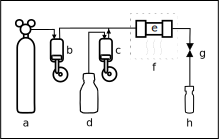
\includegraphics[width=\textwidth]{Figures/SFE_System}
\decoRule

\caption[SFE system diagram]{A diagram of an SFE system. (a) CO\textsubscript{2} supply (b)
High-pressure SF pump (c) High-pressure modifier pump (d) Modifier reservoir (e)
Extraction cell (f) Pressure control (g) Collection vessel}

\label{fig:sfediagram}
\end{figure}

\todo{Add dip tube to CO\textsubscript{2} cylinder}
\todo{Add heater to extraction cell}

Carbon dioxide (a) is readily available from suppliers of industrial gases, and
high-purity grades are available. Chromatography-grade solvents are usually used
as modifiers (d). High-pressure pumps (HPLC type) are used to compress the
carbon dioxide (b) and the modifier (c), which are mixed together at the
appropriate ratio. The mixture gets pumped into the (optionally heated (f))
extraction cell (e), which contains the material that needs to be extracted.
Having extracted the extract from the material, the supercritical fluid passes
through a pressure-control mechanism (g). This allows the pressure of the
supercritical fluid to drop to ambient, turning it into a low-density
non-solvating gas. The extract becomes desolvated, and precipitates in the
collection vessel (h). The operation of the system might be either static or
dynamic: in static operation the supercritical fluid is pumped into the system,
the flow is stopped, and the matrix/fluid mixture is given time to approach
equilibrium. Then the fluid is expelled and the extract collected.
In dynamic operation the supercritical fluid is pumped through the extraction
cell and the extract collected continuously. 


\section{Supercritical Fluid Chromatography}

An analyte will extract out of a matrix with a certain efficiency and at a
certain rate. While this is important while finding an optimum extraction
method, otherwise its relevance is limited.

However, different analytes will extract out of a matrix with different
efficiency and at different rates. In 1903 the Russian botanist Tsvet
\todo{autocite Tsvett} applied this observation to the dynamic extraction of a
bed of calcium carbonate that had an extract of plant pigments applied at the
inlet end. The different extraction efficiencies and rates of adsorption and
desorption on the calcium carbonate surface lead to the \textit{separation} of
the compounds in the mixture. Tsvet called this method of separation
\textit{chromatography}. With time this method became generalized, and today
chromatography is a major, established scientific field with many ramifications
and a myriad of applications.

Because of the different technologies used in its applications, chromatography
is conventionally classed as either \textit{gas chromatography} (GC) or
\textit{liquid chromatography} (LC). However, as we have seen, solvating gases
can also extract analytes from solid stationary phases, and hence the therm
\textit{supercritical fluid chromatography} (SFC) was created for these kind of
separations. 

Supercritical fluid chromatography as practised today bears a lot of resemblance
to \textit{high performance liquid chromatography} (HPLC). The main reason for
this is that there is a large overlap between the technology used for HPLC and
the technology needed for SFC. In particular, both use high-pressure pumps and
columns packed with particles with very small diameter, and use optical
detectors. The same instrument manufacturers who supply HPLC instrumentation
also supply SFC instrumentation.

\todo{ELSD}

\subsection{SFC and FID}

Did not always But this was not always so. In the 1980s SFC was practised using open tubular
columns and FID detectors, so the instrument designs looked more like GC instruments than HPLC instruments. 

The \textit{flame ionization detector} was invented near-simultaneously in South
Africa and New Zealand \todo{autocite FID history}. The core of the system is a
flame of hydrogen gas burning in air. The measured signal is the conductivity of
the flame plasma, which is measured by applying a -100 V potential difference
between electrodes at the tip and the base of the flame. There are very few free
ions in the hydrogen flame, so the conductivity is normally low. But organic
compounds introduced into the flame creates a number of free ions, which
increases the conductivity of the flame gases. The change in conductivity is
measured by measuring the current between the two electrodes, using an electrometer. 

The carbon dioxide in an SFC detector 

\todo{FID diagram}

The FID is quite sensitive: an x \% change in concentration will give a y \%
change in signal. This is similar to the UV detector, in which the molar
absorptivity determines the detector response. Where the FID outshines any
optical detector is in its dynamic range. The UV detector has \textit{dynamic
range} of 1000, \textit{i.e.} it can detect a 1000-fold change in concentration,
but the dynamic range of the FID detector is unsurpassed at 1000 000. This makes
the FID an excellent detector if quantitation needs to be done.

During the time SFC looked like GC, the FID was the detector of choice. But when SFC
started looking like HPLC, and the selectivity of the chromatography started
being manipulated by adding modifiers, the FID lost its utility. The quantity of modifier added to the carbon

\todos 
% Chapter 3

\begin{savequote}[60mm]
The nice thing about standards is that you have so many to choose from.
\qauthor{Andrew S. Tanenbaum}
\end{savequote}


\chapter[Biodiesel standards]{Biodiesel, technical standards and chemical analysis} % Main chapter title

\label{Chapter3} % For referencing this chapter elsewhere, use \ref{Chapter3}

The fact that vegetable oil can be used to fuel Diesel engines has been known
since the earliest days. Rudolf Diesel himself had exhibited an engine at the
Paris Exhibition in 1998 \todo{autocite Diesel peanut oil} that ran on peanut
oil. But the development of the petroleum industry late in the 19th century
ensured an ample supply of fossil fuel for these engines.

The development of the diesel engine happened in parallel with the developing
diesel fuel, for, as Cummins said \autocite{Cummins1989}``\ldots we must never
forget that \textit{an engine and the fuel it consumes are inseparable
partners}; the one cannot progress without the full cooperation of the other.''
The first invention of an engine presupposes a supply of fuel, but the drive
towards lower costs and higher efficiency then opens up the quest for more
fuels. Technically, engine builders would then have to test each new fuel in
their engines and approve of it. But fuel suppliers would like to see their
fuels used in as many engines as possible. This convergence of interests gives
rise to the establishment of \textit{technical standards}.

A technical standard or just \textit{standard} is a ``document, established by
consensus and approved by a recognized body, that provides, for common and
repeated use, rules, guidelines or characteristics for activities or their
results, aimed at the achievement of the optimum degree of order in a given
context'' \autocite{Hatto2010}. 

Standards are not mandatory, nor do they provide the `best' way of doing
something. The great strength of standards are their reliability.
``Standards exist principally to provide a reliable basis on which common
expectations can be shared regarding specific characteristics of a product,
service or process'' \autocite{BSI2016}.

Standards are published by \textit{standards organizations}, which might
be national or international in character, or might be established to serve a
certain industry. Standards organizations are often known by their
abbreviations, and a few of them are listed in Table
\ref{tab:StandardsOrganizations}. The authors of these standards documents are
usually \keyword{technical committees}, comprised of individuals from a wide
variety of stakeholder organizations, who work towards consensus.

\begin{table}
	\caption{A few well-known standards organizations}
	\label{tab:StandardsOrganizations}
	\centering
	\begin{tabular}{l l l}
	\toprule
	\tabhead{Abbreviation} & \tabhead{Name} & \tabhead{Country of origin} 		\\
	\midrule
	SABS 	& South African Bureau of Standards 		& South Africa	\\
	ISO		& International Organization for Standardization & International \\
	CEN 	& European Committee for Standardization 	& Europe		\\
	ASTM 	& ASTM International 						& USA			\\
	BSI	 	& British Standards Institution 			& UK			\\
	IEC 	& International Electrotechnical Commission & International \\
	DIN 	& German Institute for Standardization 		& Germany 		\\
	ANSI 	& American National Standards Institute 	& USA 			\\
	UL 		& Underwriter's Laboratory 					& USA 			\\
	ITU 	&International Telecommunication Union		& International \\
	\bottomrule\\
	\end{tabular}
\end{table}

Standards have a unique publication system. They are not published by publishing
houses, but by the standards organizations themselves, who sell the documents
directly to end users. Each standard is usually also better known by its number
than by its title. For example, if I were to mention the document entitled
``Quality management systems — Requirements'' few people would know that I'm
talking about the well-known quality system standard usually known as ISO 9001.

The South African national standards body is the South African Bureau of
Standards (SABS), which was established by an act of parliament,
 Standards Act, 1945 (Act No. 24 of 1945)), as amended by the Standards Act, Act
 No. 8 of 2008 \autocite{Act8-2008}. The SABS issues South African National
 Standards.

Standards organizations not only write standards, they might also
\keyword{adopt} them. Adoption happens when a suitable standard has already been
issued by another standards organization. Standards very often refer to other
standards, and standards are often based on published research. While standards
are not mandatory, some legislation might refer to 

The desire for engine designers for access to a reliable fuel and for fuel
suppliers to have the largest possible market lead them to cooperate in the
development of standards for fuels. In South Africa the relevant standard for
diesel fuel is SANS 342, and the US equivalent is ASTM D975.

Biodiesel is chemically very different from diesel, and therefore the technical
standards of biodiesel needs to be different from the standards for diesel.

\todo{Normative vs informative}

\section{SANS 1935: An overview}

The current South African standard applicable to biodiesel is ``South African
National Standard 1935 Automotive biodiesel — Fatty Acid Methyl Esters (FAME)
for diesel engines — Requirements and test methods.'' \autocite{SANS1935} This
is an adoption of the European Committee for Standardization's (CEN) standard EN
14214 \autocite{EN14214}. In the USA is the equivalent standard is ASTM D 7651,
which is largely similar but of different heritage.

SANS 1935 consists of a 18 pages. The first two pages are unnumbered: for the
purposes of this discussion they will be numbered in small Roman numerals.

\begin{description}


\item[p(i)]{The first page is a title page, following the usual format for SABS
standards. The top line of the page contains the ISBN (978-0-626-26349-2), and
in large type the standard number (SANS 1935:2011). Then follows in capital
letters ``South African National Standards'', and below that the title
``Automotive biodiesel --- FFatty Acid Methyl Esters (FAME) for diesel engines
--- Requirements and test methods''. At the bottom edge of the page we find the
SABS logo and some contact information.}

\item[p(ii)]{The second page is an informational page. It starts with a table of
changes, which was at the time of writing still empty. Then follows a foreword,
in which the committee who approved the standard is acknowledged (National
Committee SABS SC 1018A). It also gives the date of publication (December 2011)
and states that it supersedes SANS 1935:2004. Then there's very significant
line, which states that the standard is referenced in the Petroleum Products Act
\autocite{Act120-1997}. }
	
\item[p1]{Contains the Table of Contents} 

\item[p2]{Is left blank}

\item[p3]{Paragraph 1: This paragraph describes the scope of the standard, which
is that it applies to biodiesel as an automotive fuel.} 

\item[p3]{Paragraph 2:
This paragraph lists all the normative standards required to comply with to
comply with SANS 1935. Thirty-five standards are listed.} 

\item[p4]{Continues the list of normative references}

\item[p5]{Paragraph 3: This paragraph contains a list of definitions. The most
important one is this: ``biodiesel [is a] fuel comprised of methyl esters of
long chain fatty acids derived from vegetable oils.'' This is a very specific
description of biodiesel. It eliminates animal fats as a source of fatty acids,
and it excludes methyl esters. But a note reads ``Consideration for the
inclusion of ethyl esters, animal fats and C8 – C12 carbon chains should be
taken later.'' The significance of ethyl esters is that methyl esters are not
usually carbon neutral. The methanol used in the transesterification reaction is
usually obtained from the petrochemical industry, whereas ethanol from
fermentation (See Section \ref{sec:BioEthanol}) could be carbon neutral. The
definition also rules out hydrotreated vegetable oil or Fischer-Tropsch diesel
derived from biomass.}

\item[p5]{Paragraph 4: This paragraph lists requirements} 

\item[p5]{Paragraph 4.1: Discusses general requirements. According to these
requirements biodiesel is a homogeneous liquid, free of adulterants or
colourants, to which additives might be added. It prescribes testing for
oxidative stability and cold-flow properties}

\item[p6]{Paragraph 4.2: This paragraph is about physical and chemical
properties and states that biodiesel shall comply to the requirements of Table
1}

\item[p7]{Paragraph 4.3: This paragraph concerns methods of test. It states that
test methods shall be  one of the test methods listed in Table 1.}

\item[p7]{Paragraph 4.4 concerns disputes. It comes into effect when there is a
dispute about product quality between, say, a biodiesel manufacturer and a
biodiesel distributor. The contents of this paragraph prescribes which reference
method shall be used.}

\item[p7-p8]{These pages contain Table 1. The table has three columns. The first
column names a property, the second column states the numerical values it should
comply to, and the third column specify which test metod should be used to
determine that value.}

\item[p9]{Paragraph 5 describes a few simple rules for packing and marking biodiesel.}

\item[p10-p11]{Annex A describes a method for the calculation of iodine value,
which might be used instead of a measurement.}

\item[p12]{Annex B prescribes how samples for testing must be taken.}

\item[p13]{Annex C gives a list of values for calculating precision.}

\item[p14]{Annex D provides an approved method for correcting density
measurements. The prescribed tests requires density to be measured at
\SI{15}{\celsius}, which be might inconvenient. Instead, a different test may be
made at a more convenient temperature, and a correction applied. }

\item[p15]{Annex E is informative and recommends the implementation of quality
management systems. It is followed by a bibliography.}

\item[p16]{The final page contains information about the SABS and its services.}

\end{description} 

\section{SANS 1935: Properties, requirements and methods.}

On examining SANS 1935, it quickly becomes clear that the core of the document
is Table 1. This table has three columns. The first column lists a
\keyword{property}, the second column specifies a numerical value the property
has to conform to, the \keyword{requirement}, and the third column prescribes
the \keyword{test method} that must be used to obtain the value.

In the following discussion each of the requirements will be discussed, in order
of increasing relevance to this thesis, grouped by method of determination.

\section{SANS 1935: Physical methods}

\subsection{Density}

The density of biodiesel is required to be
\SIrange{860}{900}{\kilogram\per\cubic\metre} at at temperature of
\SI{15}{\celsius} The metods that can be used is described in ISO 3675 and ISO
12185. If ISO 3675 is used at a temperature other than the specified one, a
temperature correction is applied, as described in Annex D.

ISO 12185 prescribes the measurement of density by using an electronic
instrument known as the oscillating tube density meter. This measures the
density of a liquid by measuring the frequency of a tube filled with the liquid
that's oscillating freely. The frequency depends on the weight of the filled
tube, and therefore on the density of the liquid. These devices are easy to use
and very accurate. They are temperature controlled

ISO 3675 prescribes the use of a hydrometer, which is an instrument that
measures density by measuring the buoyant force on a floating indicator.
According to the law of Archimedes, the buoyant force on a body immersed in a
liquid is equal to the weight of the displaced liquid. If the liquid is denser,
the force is greater. Therefore, in a denser liquid a floating indicator would
float with more of the indicator above the surface of the liquid

\subsection{Kinematic viscosity}

The viscosity of a fluid is a measure of its resistance to flow when a force is
applied to it. Kinematic viscosity is the resistance of the flow to the force of
gravity. This flow of course depends on the density of the liquid, so that It is
important that the fuel for a diesel engine have the right viscosity, because

SANS 1935 requires that kinematic viscosity be in the \SIrange{3.5}{5.0}. The
measurement is specified by ISO 3104, which is a capillary method.

\section{SANS 1935: Aggregate properties: Specialized instrumentation}

Some of the requirements specified in SANS 1935 are not values that have direct
correspondence to physical or chemical quantities usually used in science. 

\subsection{Cetane number}

The cetane number is a number that indicates the ease of ignition of a fuel in a
diesel engine. A higher number indicates easier ignition. SANS 1935 prescribes
the test method of ISO 5165.

Cetane is a synonym for hexadecane, and is a liquid compound that ignites easily
when injected into a diesel engine. In contrast, its highly branched isomer
2,2,4,4,6,8,8-heptamethylnonane (also called isocetane) ignites less easily. The
intuitively-understood ``ease of combustion" can be quantified as the
\keyword{ignition delay}, the time between the moment when the fuel is injected
in to the engine and moment the ignition starts. A mixture of the two compounds
will have an ignition delay somewhere between that of the two compounds.

The cetane number is obtained by measuring the ignition delay in a  highly
specialized test engine. This is a single-piston, four-stroke engine that has a
combustion chamber of variable volume, which gives it a variable compression
ratio. While running on the fuel under test, the compression ratio is changed
until a prescribed ignition delay is achieved. Then the cetane/isocetane mixture
that will give the same ignition delay at that compression ratio is found. If
the fuel under test has the same ignition delay as a pure cetane, it is assigned
the cetane number of 100. If it has an ignition delay that is the same as
isocetane, then the cetane number 0 is assigned, and if it has the same ignition
delay as a 50:50 cetane:isocetane mixture, then it is assigned the cetane number
of 50.

Cetane number gives limited insight into the chemical properties of the fuel, or
indeed, engine performance. But it is a trusted measure of the suitability of a
fuel for use in a diesel engine. 

\subsection{Flash point}

Fuels are, naturally, flammable, and different fuels are flammable to different
degrees. A fuel's \keyword{flash point} can be used to quantify its degree of
flammability. The flash point is the temperature at which a fuel's vapour will
ignite when it comes in contact with a flame. 

The measurement of flash point is not primarily concerned with the performance
of the fuel inside the engine, but is important to know because it determines
how the fuel can be safely be handled during transport and storage
\autocite{WFCC2009}.

The flash points of liquids are established by standardized tests in automated
apparatus.

\subsection{Oxidation stability}

Fossil fuels for diesel engines are largely composed of alkanes, which are
chemically very inert. This means that they can be stored for long periods
without significant degradation.

Biodiesel, by contrast, are by definition (\autocite[Paragraph 4.1.1]{SANS1935})
mostly composed of fatty acids by definition, which are not inherently stable.
This instability has been known since antiquity as fatty food going
\keyword{rancid}. In particular, double bonds in the fatty acids are liable to
reactions with atmospheric oxygen \autocite(Velasco2010). These are free radical
reactions, illustrated in Figure \ref{fig:RancidRadical}.

\begin{figure}
\centering
\includegraphics[width=\textwidth]{Figures/1281px-Lipid_peroxidation.svg.png}
\decoRule

\caption[The peroxidation of lipids.]{The peroxidation of lipids. By Tim
Vickers, after \autocite{Young2001}. - w:Image:Lipid peroxidation v2.png, Public
Domain, https://commons.wikimedia.org/w/index.php?curid=1728531}

\label{fig:RancidRadical}
\end{figure}


\todo{The reaction products are short-chain fatty acids, soaps, sludges.}

The oxidative stability is measured by the Rancimat, an automated instrument. It
works by bubbling a stream of hot air through a sample of biodiesel. This air is
then passed through a conductivity measuring cell filled with distilled water.
The conductivity of the water increases when volatile acids dissolves in it. At
the beginning of the test period there are very few acids dissolved swept into
the water, so the conductivity remains low. As the sample oxidizes and produce
acids, the conductivity of the water slowly increases. But the oxidation
reaction is \keyword{autocatalytic}, which means that the products of the
oxidation reaction accelerates the oxidation. The result of the autocatalysis is
that on the conductivity curve there is a sudden increase in conductivity. The
time taken until this point is reached is called the \keyword{induction period}.

SANS 1935 requires a minimum induction period of 6 minutes at 110
\SI{110}{\celsius}. Paragraph 4.1.2 permits the addition of antioxidants.

\subsection{Cold filter plugging point}

The flow of liquids depend on the temperatures. Most obviously, their densities
depend on the temperature. But liquids can freeze, which will also influence
their flows. Inside an engine at operating temperature the temperature of the
fuel will be high enough, but the biodiesel needs to be pumped to the engine
from the fuel tank, passing through a fuel filter on the way. If crystals of
fuel form at low temperatures, these crystals might plug the pores in the
filter, which could lead to fuel starvation in the engine. It is therefore
important that the biodiesel must be able to be pumped through the engine's fuel
filter at all expected temperatures.

For this purpose SANS 1935 specifies a \keyword{cold filter plugging point}. It
is the lowest temperature at which a given volume of biodiesel still passes
through a standardized filtration device in a specified time when cooled under
certain conditions. This is an entirely practical test: no fundamental
physical property is measured.

\section{SANS 1935: Chemical properties: Classical determination}

\subsection{Sulfated ash}

Ash is the solids remaining after the complete combustion of a fuel. This means

\keyword{Sulfated ash} is the residue remaining after the lubricating oil sample has been
carbonized, and the residue subsequently treated with sulfuric acid and heated
to constant mass.



\subsection{Carbon residue}

\subsection{Total contamination}

\section{SANS 1935: Chemical properties: Electrochemical determination}

\section{SANS 1935: Chemical properties: Spectroscopic determination}

\section{SANS 1935: Chemical properties: Chromatographic determination}

\section{Petroleum Products Act}

SANS 1935 is referred to in the Petroleum Products act, which makes it illegal. 

\section{Fast Gas Chromatography}

\todo{autocite Blumberg 1997}
% Chapter 4it

\begin{savequote}[\quotewidth]
$pV \neq nRT$ 
\qauthor{The universal gas law does not apply to supercritical fluids}
\end{savequote}

\chapter{Instrumentation: Supercritical Fluid Chromatography} % Main chapter title

\label{Chapter4} % For referencing this chapter elsewhere, use \ref{Chapter4}

In this thesis the development of a comprehensively coupled (supercritical fluid
× gas) chromatograph and its application to the analysis of biodiesel is
discussed. The discussion on the experimental work divides naturally into two
parts: this chapter discusses the supercritical fluid chromatography (SFC) and
the next chapter discusses the gas chromatography (GC).

\section{SFC}

As discussed in Chapter \ref{Chapter2}, an SFC chromatograph consists of a
supply of mobile phase, a pump, a pressure control system, a modifier control
system, a column, a pressure relief system and a detector. These subsystems are
discussed below.

\section{Mobile phase}

As mobile phase we used carbon dioxide. The benefits of carbon dioxide as an
solvent and mobile phase is discussed in Chapter \ref{Chapter2}. We used
\SI{99.995}{\percent} pure carbon dioxide supplied by Air Products. Our
colleagues in industry also use food grade or technical grade carbon dioxide and
they have not reported any significant impurities.

As modifier we used LiChrosolv\textregistered methanol from Merck. This is an
`HPLC-grade' solvent, of which the purification is optimized for the removal of
UV-absorbing impurities. Using this grade of solvents is important when using
optical absorbance or fluorescence detectors, because lowering levels of
impurities improve limits of detection. It is quite likely that a less expensive
grade of modifier would also be suitable for our SFC, because we do not use an
optical detector.

\section{Pump}
\label{sec:CO2Pump}

As pump we used the robust, reliable Varian 8500 HPLC pump because it was
available. This pump had its control electronics removed, and it was controlled
from a personal computer by software written for the purpose. The Varian 8500
pump is driven by a stepper motor. This kind of motor turns in discrete steps,
instead of at a constant rate. It is driven by pulses of electric current,
rather than a continuous current, and therefore the speed of the motor can be
controlled by varying the rate of the pulses. This makes it relatively simple to
control the speed of the motor from a computer. The Varian 8500 pump has a
built-in pressure transducer that provides an electronic signal proportional to
the pressure at the pump outlet.

The Varian 8500 pump is a single-piston pump with a \SI{250}{\milli\litre}
capacity that needs to be refilled between strokes. Refilling means that one has
to stop chromatography, which makes it important to fill the pump to full
capacity, so that chromatographic runs are not interrupted. This means that the
pump needs to be filled with carbon dioxide in the liquid phase rather than the
vapour phase. Compressing either would create the appropriate phase for doing
chromatography, but compressing a vapour would leave one with a much smaller
volume of high-pressure carbon dioxide than compressing a liquid. Filling a pump
with liquid carbon dioxide is more difficult than one might imagine.

\begin{figure}
\centering
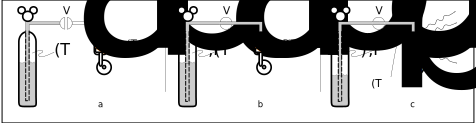
\includegraphics[width=\textwidth]{Figures/CO2Filling.pdf}
\decoRule

\caption[Filling a CO\textsubscript{2} pump.]{A schematic diagram of the process
of the filling of the carbon dioxide pump. (a) The pressure in the reservoir
$P_a$ is much higher than the pressure in the receptacle $P_b$. The valve is
closed, so there is no flow. (b) The valve is open and some carbon dioxide has
flowed from the reservoir to the receptacle. But $P_b = P_a$, so there is no
flow. (c) When the temperature in the receptacle $T_b < T_a$, then $P_b  < P_a$,
following Gay-Lussac's law. Flow will continue until all the vapour in the
receptacle has condensed.}

\label{fig:co2fill}
\end{figure}


Imagine a reservoir of liquid carbon dioxide, equipped with a dip tube,
connected to an empty receptacle via a valve (V). (See Figure \ref{fig:co2fill})
One can assume that the receptacle is empty and contains only carbon dioxide
vapour at atmospheric pressure, say \SI{1}{\bar}. The vapour pressure of the
vapour above the liquid in the reservoir is about \SI{55.3}{\bar}
(\SI{5.6}{\mega\pascal}). When the valve (V) is opened the will high-pressure
vapour in the reservoir will expel the liquid carbon dioxide through the dip
tube and through the valve, into the receptacle. In the low-pressure environment
of the receptacle the carbon dioxide will boil. Soon there will be some liquid
carbon dioxide in the receptacle, with the rest of the receptacle volume filled
with gaseous carbon dioxide. When the system comes to equilibrium the pressure
in the receptacle ($P_b$) will equal the pressure in the reservoir ($P_a$), and
there will be no flow of liquid carbon dioxide. One can attempt to now increase
the flow by increasing the volume of the receptacle (for example by withdrawing
a pump piston), and hence decreasing the vapour pressure there. But any flow
from the reservoir will lead to expansion of the headspace of the reservoir.
This will lead to cooling of the vapour, and therefore lower pressure and
therefore lower flow. The final result of this process is that the receptacle is
never filled to capacity with liquid.

The only way to restore the flow from the reservoir to the receptacle is to
create a pressure difference $P_a - P_b$. While it is possible to create an
overpressure in the reservoir by adding a headspace gas, it is technically
challenging and expensive. It is simpler to use the Gay-Lussac gas law.
According to this law the ratio of the pressure to the temperature of a gas is
constant so that $\frac{P_b}{T_b} = k$. This means that a decrease in
temperature will lead to a decrease in pressure. The way to fill the reservoir
to capacity is to ensure that the temperature of headspace vapour $T_a$ is higher
than the temperature of the headspace vapour $T_b$. Because safety regulations
prohibit the heating of a cylinder of pressurized gas, the way to ensure $T_a <
T_b$ is to cool the receptacle. This cools the headspace vapour, and following
the Gay-Lussac law the pressure $P_b$ decreases, the difference $P_a - P_b$
increases and the liquid flows until the receptacle is filled to capacity.
 
In the case of the Varian 8500 pump the cooling of the pump was achieved by
wrapping a coil of copper tubing around the cylinder, and pumping a chilled
heat-exchange fluid through it. A chiller with a mechanically cooled tank with a
\SI{20}{\litre} capacity was filled with a solution of \SI{5.0}{\litre} of
diethyl glycerol in about \SI{10}{\litre} of water. This mixture has a freezing
point of \SI{-15}{\celsius}, which can be cooled by the chiller without
freezing. (If the coolant freezes a layer of ice forms on the cooling plate of
the chiller, which isolates the remaining liquid from the cooling plate and
limits the minimum temperature of the coolant.) An inexpensive submersible water
pump (designed for decorative water fountains) was used to pump the coolant
through the circuit. This pump can deliver \SI{800}{\litre} of water per hour at
a head of \SI{1.2}{\metre}.

For some experiments we also used a SFT-10 pump from Supercritical Fluid
Technologies (Newark, Delaware). This is a purpose-built two-piston pump with
sapphire valve seats and a Peltier-cooled head. This is a much better technology
than the HPLC pumps. It takes up less space and does not need refilling, since
it feeds directly from the cylinder. This pump had its own microprocessor
controllers on board, and flow and pressure could simply be commanded from the
PC through a USB cable.

\subsection{Pressure control system}

The aim of chromatography is to separate chromatograms by a certain distance.
But the days of separating coloured compounds in glass packed columns are long
past and the direct measurement of distances are now relegated to thin-layer
chromatography. Instead, we have to make do with proxies for distance such as
\keyword{retention volumes} or \keyword{retention times}.


% In chromatography the figure of merit by which the performance of a system is
% measured is the distance by which two compounds are separated, relative to their peak
% widths. This is known as the \textit{resolution}. 

Retention times are particularly convenient today, because they can easily be
measured by computer systems. Retention times, however, depend on a known flow
rate of the mobile phase through the column. The flow rate need not be constant,
although for the sake of simplicity a constant flow rate is preferred. Ideally,
the flow rate should also be adjustable. The need for an adjustable, constant
flow rate can be met by using a control system. Control systems are well
understood by engineers, among whom it is a major field of study
\autocite{Koenig2009}.

Figure \ref{fig:processcontrol} shows a diagram of a simple process control
system. Some aspect of the process under control is measured, which yields the
\keyword{process variable} (PV). The PV is compared to the \keyword{set value}
(SV), and the \keyword{error} (e) is obtained by finding the difference. The error
is provided to the controller, which calculates the \keyword{manipulated
variable} (MV). The MV is used to drive the final control element, which adjusts
the process with the aim of producing a smaller error.

\begin{figure}
\centering
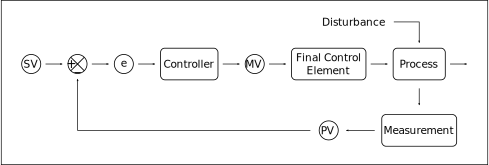
\includegraphics[width=\textwidth]{Figures/ProcessControl.pdf}
\decoRule

\caption[A process control system]{Schematic diagram of a closed-loop control
system. (SV) Set Value, (PV) Process Variable, (e) Error, (MV) Manipulated
Variable}

\label{fig:processcontrol}
\end{figure}

Chromatographic systems conventionally work under pressure control or flow
control regimes. Either is suitable: constant pressure systems usually yield
constant flow if other parameters are held constant. Because flow measurement is
more complex than pressure measurement, pressure control is the older, simpler
and less expensive control method. Also, in SFC the solvent strength of the mobile
phase is pressure/density dependent. We therefore selected pressure control
as our control regime.

In our system the pressure measured by the on-pump sensor was the process
variable (PV) . This was compared to the set value (SV) set on the computer
console. The controller was a software algorithm, implemented as a virtual
instrument in the programming environment LabVIEW. The controller computed an
output value for the manipulated variable (MV), which was the rate at which
pulses were sent to the pump, in hertz. The digital input/output (DIO) interface
of a National Instruments PCI-6014 multifunction data acquisition board created
those pulses and sent them to the pump's electronic interface.

The software used a PID (Proportional-Integral-Derivative) controller module,
with the Integral and Derivative contributions disabled. The simpler
proportional control was found totally adequate for our purpose, and it can be
improved in future by finding an appropriate tuning method and applying it with
the integral and/or derivative activated.

% While enabling the Integral and Derivative contributions would add to the
% accuracy of the controller, we could not find a suitable, simple tuning
% procedure.

% Tuning the controller from adequate performance to optimum performance would
% consume resources while not improving the chromatography.

\subsection{Modifier Control}

The modifier needs to be present in the mobile phase at a known and controlled
concentration. There are various SFC-modifier mobile phase supply units on the
market. They tend to be expensive and complex, because they require the use of
two controlled, high-pressure pumps. Given that our needs were rather modest, we
elected to use a simpler system. Instead of accurately pumping the supercritical
fluid and the modifier, we only pump and control the supercritical carbon
dioxide and add measured volumes of modifier.

The modifier control unit consisted of a six-port valve, a fixed-volume
measuring loop, and a mixing chamber. The unit operates by filling the measuring
loop with modifier, and then switching the measuring loop into the flowing
mobile phase. The modifier is washed into the mixing chamber, where it is
intimately mixed with and dissolved in the supercritical carbon dioxide. The
concentration of modifier in the mobile phase is determined by the switching
rate of the sampling valve. Given that about 3 volumes of supercritical carbon
dioxide is needed to wash the modifier out of the loop, the highest
concentration of modifier that can be added in this manner is about
\SI{25}{\percent}.

Figure \ref{fig:mixingchamber} shows the chosen design of the mixing chamber.
The inlet and outlet pipes of the mixing chamber extend far into the chamber, to
break up plug flow and encourage rapid mixing.  

\begin{figure}
\centering
\includegraphics[width=\textwidth]{Figures/MixingChamber.png}
\decoRule

\caption[A cutaway diagram of the mixing chamber]{A cutaway diagram of the
mixing chamber design. The chamber is designed for the mixing of the modifier
and the supercritical carbon dioxide.}

\label{fig:mixingchamber}
\end{figure}

The modifier injection valve position was commanded from the controlling PC by electronic
voltage pulses.

\section{Sample injection}
\label{sec:SFCInjection}

The sample inlet was a two-position rotary valve with an internal sampling
volume (Figure \ref{fig:samplingvalve}). In one position the sampling volume is
filled with a syringe, and when the valve was commanded to inject the sampling
volume is switched into the carrier mobile stream. The sample volume was
\SI{0.5}{\micro\litre}. The injection valve position was commanded from the
controlling PC by electronic voltage pulses.

\begin{figure}
\centering
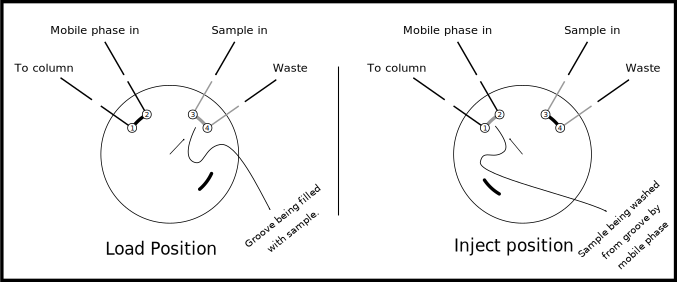
\includegraphics[width=\textwidth]{Figures/SampleValve.pdf}
\decoRule

\caption[Schematic diagram of the injection valve.]{A schematic diagram of the sampling valve. }

\label{fig:samplingvalve}
\end{figure}

The reader might be more familiar with the six-port valve as an injection
system. The benefit of the internal groove injection valve is that it allows a
much smaller volume to be injected. Using this small volume makes it possible to
inject samples without dilution, which simplifies sample preparation. A drawback
of this design is that it is not possible to vary the volume of sample injected.


\subsection{Column}
\label{sec:SFCColumn}

The separation power of a chromatographic system can be modelled by the equation 

\[
 R_s = \left(\frac{\sqrt{N}}{4}\right)  \left(\frac{\alpha-1}{\alpha}\right)  \left(\frac{k'}{1+k'}\right)
\]

were \(R_s\) is the \keyword{peak resolution}, \(N\) is the \keyword{number of
plates}, \(alpha\) is the \keyword{selectivity}, and \(k'\) is the
\keyword{retention factor}.
 
The number of plates \(N\) can be increased simply by making the column longer,
at the cost of increasing the time of the run. The maximum length of the column
is determined by the pressure drop available that will still yield adequate
flow. In capillary gas chromatography the openness of the column and the low
viscosity of the gas-phase mobile phase routinely allows columns \SI{100}{\metre
}long at inlet pressures of a few atmospheres. In HPLC the high viscosity of the
mobile phase and the narrow, tortuous pathways between the small particles of
the packing material means that the columns are typically
\SIrange{100}{200}{\milli\metre} long, requiring hundreds of atmospheres of
inlet pressure for adequate flow.

The low viscosity of an SFC mobile phase allows operation of much longer
HPLC-type packed columns. This provides a much higher number of plates in the
chromatographic system than HPLC. The SFC column we used in the SFC×GC system
was a set of five HPLC columns (\SI{150}{\milli\metre} $\times$
\SI{4.6}{\milli\metre}, \SI{3}{\micro\metre} particles) (Restek, Pinnacle DB
Silica) connected in series.

The stationary phase in this column is `bare silica', which is usually
considered 'polar'. That means that the packing of the column consists of porous
silica particles with no organic phase covering its surface, and hence one that
will interact strongly with polar molecules. In contrast, the ubiquitous `C18'
stationary phase used in reverse-phase HPLC is 'non-polar'. The particles of
such a stationary phase are coated with octadecyl chains bonded to its surface,
and hence will tend to interact strongly with non-polar molecules. The base
material of the particles is usually silica, but that is only because
manufacturing uniform particles of a given size from silica is a mature
technology and not because silica is important to the separation mechanism. (In
fact, some care has to be taken to deactivate the silica so that it does not
contribute to the retention. Such a mixed retention mechanism can lead to
\keyword{peak tailing}.)

\subsection{Stopped-flow}
\label{sec:stopflow}

Among analytical chemists it is the convention that chromatographic runs are
done without interruptions. In our SFC×GC chromatograph we collect fractions of
SFC eluate and separate them by GC. It is possible to collect, store and inject
fractions of SFC eluate while maintaining continuous flow, for example using a
dual storage loop system like the one depicted in Figure
\ref{fig:continuousflow}. But such systems require careful selection of volumes,
fraction collection reservoirs with matching volumes, and an auxiliary pump.

\begin{figure}
\centering
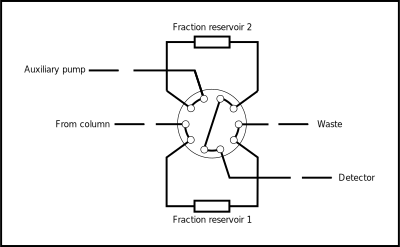
\includegraphics[width=\textwidth]{Figures/ContinuousFlowStopValve.pdf}
\decoRule

\caption[Schematic diagram of a continuous-flow valve.]{A schematic diagram of a
valve configured to allow continuous-flow fraction collection. }

\label{fig:continuousflow}
\end{figure}

Instead of such a system, we opted for a more versatile and simpler stopped-flow
system. In this system a fraction of the SFC eluate is collected, and then the
flow through the column is stopped. While the flow is stopped the collected
fraction is subjected to separation by GC. The flow was stopped by a six-port
rotary valve using three of the ports, directing flow either to a blocked-off
port or to the depressurizer, in effect making it an on-off controller.

In packed columns, "eddy diffusion is always the main cause for peak broadening
at any temperature and at high velocities" \autocite{Gritti2006}. During the
period that the flow is stopped only longitudinal diffusion contributes to peak
broadening, which is small compared to eddy diffusion in dense mobile phases.
Using the simple stopped-flow technique of sample collection will therefore not
have a major effect on the resolution of the \oneD chromatography.


\section{Pressure Relief}
\label{sec:Restrictor}

No matter the kind of SFC system one uses, at some point the eluate needs to be
depressurized. This can be before or after the detector. If depressurization
happens after the detector, then the details of the mechanism doesn't matter
much, because the information has been obtained and the eluate can be discarded.
If, as in our case, the depressurized eluate needs to still pass the detector,
it is important to not lose the resolution achieved by the column.
This means that the design of the depressurizer requires some care.

The main concern in depressurizer design is premature desolvation of analytes.
This causes \keyword{discrimination}, which is the differential treatment of
substances where identical treatments are required. In particular, compounds of
higher molecular weight tend to desolve first from the supercritical fluid, and
might precipitate in the wrong place if the depressurizer is not designed to
prevent it. 

Depressurization can be done either statically or dynamically. In a dynamic
system there is an active element that controls the flow of the eluate in such a
way as to maintain the pressure upstream of the active element of the
controller. Such a device is often called a \keyword{back pressure regulator},
and is usually an electromechanical device with digital control. They tend to
be complex and expensive.

In static depressurization there is no active pressure control. A simple
\keyword{restrictor} is used to limit the flow between the high pressure of the
SFC and the low-pressure outlet. Textbooks often discuss different restrictor
designs. \autocite[The book by][provides an example.]{LuquedeCastro1994}. Our
preferred depressurizer was the `integral' or Guthrie design
\autocite{Guthrie1986}. Figure \ref{fig:restrictor} shows the steps in
manufacturing the Guthrie restrictor.

\begin{figure}
\centering
\includegraphics[width=0.5\textwidth]{Figures/Restrictor.pdf}
\decoRule

\caption[A diagram of a integral restrictor.]{The steps of making a Guthrie restrictor. (a) Cut
length of quartz capillary (b) Heat with flame to soften glass and create
internal cone (c) Grind down end to expose orifice of the appropriate size.}

\label{fig:restrictor}
\end{figure}

We found this restrictor robust and fairly simple to manufacture. It was
possible to adjust the flow to a given flow rate. This design of restrictor
should eliminate discrimination, because the decompression takes place in a very
short space.

However, the Guthrie design proved prone to blockage. These blockages could not
be eliminated by incorporating a \SI{0.5}{\micro\metre} filter before the
restrictor, which prompted an investigation into the cause of blockages. To rule
out the possibility that it was particles that caused the Guthrie restrictor to
become blocked, we first had to determine the diameter of the orifice. This
proved to be harder than expected: optical microscopy was not able to give a
simple, unambiguous measure of the orifice diameter. Scanning electron
microscopy (SEM) showed that the orifice diameter of a Guthrie restrictor is
about \SI{10}{\micro\meter}, as shown in Figure \ref{fig:restrictororifice} This
makes it very unlikely that particles with an origin in the SFC system blocked
the restrictor: even the \SI{3}{\micro\meter} particles from the column packing
material should not block this restrictor.

\begin{figure}
\centering
\includegraphics[width=\textwidth]{Figures/sem_h_001.png}
\decoRule

\caption[A electron microscope photo of a restrictor orifice]{An electron
micrograph of a restrictor tip, showing the size of the orifice.}

\label{fig:restrictororifice}
\end{figure}

Experience had taught us that the restrictor did not block if the flow was
continuous. It was only when the pressure in the restrictor cycled that
blockages occurred. To eliminate the possibility that it was material from the
stop valve (see Section \ref{sec:stopflow}) that caused the blockages, we cycled
the pressure by switching the pump on and off, allowing the pressure to bleed
off through the restrictor. This way of cycling the pressure did not prevent
blockages.

Examining the blocked restrictors with an electron microscope revealed that the
restrictors became blocked by a soft material. Backscatter SEM mode allows the
energy of X-rays to be measured by energy-dispersive spectrometry, which yields
information about elemental composition. While much care must be taken before
this information can be used for quantitation, it revealed that the deposited
material contains significant quantities of carbon and oxygen, and possibly some
chlorine. This points to the probability that the material blocking the column
is organic in nature, and possibly polymeric. See Figure
\ref{fig:restrictorblockage}.

\begin{figure}
\centering
\includegraphics[width=\textwidth]{Figures/Blockage_1920.png}
\decoRule

\caption[A electron microscope photo of a blocked restrictor orifice]{An
electron micrograph of a blocked restrictor orifice. (a) Original
image (b) Image with black circle showing estimated original orifice location}

\label{fig:restrictorblockage}
\end{figure}

We could not determine the origin of the material, but it seems likely to be the
column, because cycling the pressure without a column did not cause a blockage.
We eliminated the possibility of blockage by sample material by using a brand
new column. We suspect that the blocking material might be remnants of
surfactants used in the synthesis of the silica gel stationary phase. These
surfactants are leached out of the column packing by the highly diffusive
supercritical fluid mobile phase, and they then precipitate in the restrictor
when the pressure drops and the compounds desolvate. Repetitive pressure cycles
causes a build-up of material which gradually blocks the orifice.

The smallness of the orifice contributes to the plugging problem. With a
diameter of \SI{50}{\micro\metre}, a solid sphere that fits in this capillary
will have a volume of \SI{0.065}{\nano\litre}, or \SI{65}{\pico\litre}. This
means that nanogram quantities of material can easily block the restrictor.

Being satisfied that an unfortunate combination of restrictor design and column
packing was the likely cause of the blockages, we chose a different restrictor
design. The choice was a simple linear restrictor and we trusted that heating
the end of the restrictor would prevent discrimination. The final linear
restrictor was \SI{800}{\milli\metre} long and had an internal diameter of
\SI{0.050}{\milli\metre}.

\section{Detector}

When SFC was first developed, a capillary column was the usual column, and an
FID was the usual detector. In current use, however, packed columns used with
mobile phase modifiers predominate and flame detectors have lost their place:
the high concentration of modifiers in the mobile phase would swamp the signal
from analytes or saturate the detector. Therefore modern SFC uses predominantly
UV/Vis optical detectors.

In the supercritical fluid chromatograph described in this chapter there was no
dedicated detector: the role of the detector was taken by a gas chromatograph.
This gas chromatograph collected fractions from the SFC, and separated them in
fast chromatographic runs with an FID detector, yielding comprehensive 2D
chromatograms. This chromatograph-as-a-detector is described in Chapter
\ref{Chapter5}.
 
% Chapter 5

\begin{savequote}[45mm]
I feel the need \ldots the need \ldots for speed\ldots
\qauthor{Top Gun}
\end{savequote}

\chapter{Instrumentation: Fast temperature programmed gas chromatography} % Main chapter title

\label{Chapter5} % For referencing this chapter elsewhere, use \ref{Chapter5}

A gas chromatograph consists

\section{Main Section 1}

\subsection{Subsection 1}

\subsection{Subsection 2}

\section{Main Section 2}
 
% Chapter 6

\begin{savequote}[45mm]
Coconut oil for your skin \ldots
\qauthor{Polynesian proverb}
\end{savequote}

\chapter{Investigating biodiesel feedstock by SFC×GC} % Main chapter title

\label{Chapter6} % For referencing this chapter elsewhere, use \ref{Chapter6}


\section{Introduction}

Biodiesel is composed of a mixture of methyl esters of fatty acids obtained from
plant oils \autocite{SANS1935}. To comply with the relevant standard
\autocite{SANS1935}, (See chapter 3), it must consists of a mass fraction of
\SI{96.5}{\percent} or more of methyl esters, and it must have fewer than a
certain amount of specific unsaturated fatty acids methyl esters.

The methods for determining fatty acid methyl esters are chromatographic. Each
limit has its own method, and it therefore becomes expensive to determine each
of them.
 
Both these methods generate complex chromatograms that need highly skilled and
experienced chromatographers to interpret. Each peak in the chromatogram has a
retention time and area, which needs to be interpreted. There is no doubt that
the use of artificial intelligence and other technological innovation for
interpreting chromatograms will grow \todo{Cite AI chromatogram
interpretation.}, but the paradox of automation (automation helps you least when
you need it most\todo{autocite Automation paradox Strauch2018 Bainbridge1983})
predicts that as biodiesel production grows, with the implied increase in
complexity as feedstocks differentiate, the analytical chemist will need better
chemistry, in addition to better automatic data analysis.

Comprehensively coupled chromatography offers a way to better exploit chemistry
for improved separations. It does this in three ways: the first is increasing
the peak capacity of the system, the second is by improved sensitivity, and the
third is by generating patterns in the data.


\section{SFC of FAMEs}

The power of comprehensive chromatography is unlocked by orthogonality.
Orthogonality is the difference is separation mechanism in the two dimensions
\todo{autocite{LGGC nomenclature}}. When fatty acid methyl esters are separated
by a system using pure carbon dioxide as a mobile phase and unmodified silica as
a stationary phase, then the separation is according to the number of double
bonds, independent of chain length \autocite{Robertson1991, Smith1994,
Smith2001}. This is in strong contrast to the separation of FAME by GC, where
the major separation is according to volatilty, which can be adjusted, but not
overridden, by changing the polarity (or other chemical aspect) of the mobile
phase.

\begin{figure}
\centering
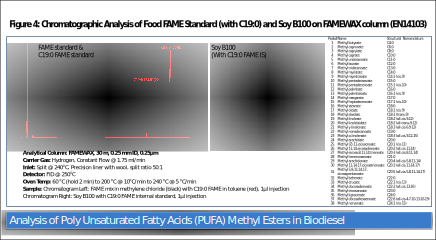
\includegraphics[width=\textwidth]{Figures/FAME-GC.pdf}
\decoRule

\caption[Separation of FAME by GC]{This figure shows that when separating FAME
by GC, using specialized column, separation is primarily by fatty acid chain
length, and secondarily by number of double bonds.The peaks elute }

\label{fig:co2fill}
\end{figure}

Silver ions are often used in stationary phases to separate unsaturated
compounds, and this includes stationary phases for SFC \autocite{Sandra2002,
Potgieter2013}. The retention mechanism is quite complex
\autocite{Nikolova-Damyanova2019}, but it offers a powerful technique for the
elucidation of lipid structures, as reviewed as early as 1966
\autocite{Morris1966}. Nevertheless, in this chapter the use of stationary
phases modified with silver ions was neither necessary nor attempted.

The low viscosity of the carbon dioxide mobile phase allows for the use of very long
columns \autocite{Smith2001}.

As discussed in Section \ref{sec:Rancimat}, fatty acids are not stable at high
temperatures. This means that they might degrade during chromatographic
separation at high temperature, especially if the run times are long. Because
SFC operates at low temperatures, the labile compounds are less likely to degrade. 

\section[Benefits of fast GC]{Benefits of fast temperature programming GC for FAME analysis}

As discussed in Section \label{sec:ChromDet}, FAME can be separated by gas
chromatography using a relatively non-polar columns with high-temperature
programs. For this purpose column manufacturers supply special 'high
temperature' columns, which address two aspects of column lifetime: mechanical
degradation and stationary phase degradation. 

Fused silica has a high \keyword{tensile strength}, but also a low
\keyword{fracture toughness}. This means that it is strong enough to resist the
forces involved in its use as a column, but very liable to fracture if it gets
damaged. Very small flaws, less than a micron in depth, will cause fused silica
(or any other glass) to fracture under loads far under what would be expected
from it's tensile strength. Such flaws can be caused by mechanical scratches or
reaction with atmospheric water. Therefore the fused silica capillary is coated
in a layer of polyimide, which protects it from environmental damage. The
strength of the a capillary column therefore depends strongly on the integrity
of the polyimide coating. The polyimide, like all resins and polymers, degrade
faster at higher temperatures, so the longer the column spends at high
temperature, the shorter the overall mechanical lifetime of the column will be.
Temperature programs that minimize the time spent at high temperature will
therefore contribute to longer column lifetimes.

Column mechanical lifetime can also be improved by using metal capillaries.
Metals are not afflicted by brittle fracture the way fused silica is, but they
don't offer the chemical inertness of fused silica. But technologies have been
developed to deactivate metal surfaces \autocite{Smith2002}, which made metal
columns a modern possibility. Column manufacturers offer metal columns
specifically designed for biodiesel analysis.

Column manufacturers' high-temperature columns also minimize stationary phase
degradation by using highly cross-linked resins, or polymers with backbones
resistant to certain degradation mechanisms \autocite{Day2003}.

\todo{Include column bleed mechanism?}

Short columns and fast temperature programs have a beneficial side effect:
reduced \keyword{column bleed}. Any resin- or polymer-based stationary phase
degrades over time, and this degradation is faster at higher temperatures
\autocite[p. 66]{Mcnair2019}. It is observed as a rise in baseline during the
high temperature part of a temperature program. Various stationary phase
technologies can be employed to reduce column bleed, but it should be obvious
that a \SI{1}{\metre} column will have \num{1/30}th \todo{fix ordinal} of the
column bleed of a \SI{30}{\metre} column. (It should be noted that the column
lifetime will not be longer, just that the increase in baseline signal from
column bleed will be lower.)

Another durability benefit of the coaxial stainless steel heater is that the
outer surface of the capillary column is protected from mechanical damage by
being encased. During development of the coaxial heater there were occasions
where the column was accidentally overheated by poorly-controlled resistive
heating. Even though the polyimide coating had been completely charred away and
the capillary was fragile, the column was intact and still provided good
separations.

Using carbon dioxide as coolant also protects the polyimide coating from
oxidative damage by purging the column environment of oxygen.

An aspect of fast temperature programming with such a temperature range as we're
using (\SIrange{-30}{400}{\celsius}) is \keyword{thermal shock}. Thermal shock
occurs when an object is subjected to a rapid change in temperature. Under such
non-equilibrium conditions different parts of the object will have different
temperatures. The material that the object is made of has a certain
\keyword{coefficient of thermal expansion}, which means that the relative sizes
of parts of the object will differ. This will cause stress between the parts,
and if the stress exceeds the strength of the material, the material might
fracture. Fused silica has a low coefficient of expansion \todo{autocite}, and
therefore low thermal shock, and the amount of material in a capillary is
relatively small, so we have never seen a column fail due to thermal shock.

Apart from thermal shock, there is also \keyword{thermal fatigue}. ``Thermal
fatigue (TF) is the gradual deterioration and eventual cracking of a material by
alternate heating and cooling during which free thermal expansion is partially
or completely constrained'' \autocite{Rao2001}. The expansion of the portion of
the fused silica column subjected to alternate heating and cooling is not
constrained, and the part of the fused silica column that is constrained (in the
sealing ferrules) is not subjected to alternate heating and cooling (it is held
at constant temperature in the heated T-piece block) therefore we do not expect
thermal fatigue. We did not explicitly test for the occurrence of thermal
fatigue, but we have not observed column failure due to thermal expansion.

One failure of the coaxial heater could be attributed to corrosion. The joint
between the coaxial heater and the heated T-piece block is brazed, and there was
a failure of the thin-walled stainless steel tube near that joint, in the
portion heated during the brazing operation. Visual inspection seemed to
indicate thinning caused by corrosion. Acid flux was used, which might have
contributed to the corrosion.

\section{Experimental}


\subsection{Samples}

Various samples of vegetable oil for were obtained from supermarkets. (See Table \ref{tab:OilSamples})

\begin{table}
	\caption{Oils used for FAME analysis}
	\label{tab:OilSamples}
	\centering
	\begin{tabular}{l l l}
	\toprule
	\tabhead{Abbreviation} & \tabhead{Name} & \tabhead{Country of origin} 		\\
	\midrule
	Oilve oil 	& 	Oilve oil 	& South Africa	\\
	Coconut oil	&  	Oilve oil & International \\
	Sunflower oil	& European Committee for Standardization 	& Europe		\\
	\bottomrule\\
	\end{tabular}
\end{table}

 
% Chapter 7

\begin{savequote}[45mm]
Modified\ldots
\qauthor{Ancient proverb}
\end{savequote}

\chapter{Application: Modified SFC} % Main chapter title

\label{Chapter7} % For referencing this chapter elsewhere, use \ref{Chapter7}

%----------------------------------------------------------------------------------------
%	SECTION 1
%----------------------------------------------------------------------------------------

\section{Introduction}

Modifiers in SFC are incompatible with FID, but if you add a fast CG as a
detector, then the volatile modifier is separated from the analytes, and the
modifier elutes as a solvent front, leaving the GC peaks uninterfered with.


\section{(Modified SFC)×GC}

\subsection{Sample}

\subsection{SFC}

\subsection{Modulation}

\subsection{GC}

\subsection{Results}

See Figure \ref{fig:Modifier}

\begin{figure}
	\centering
	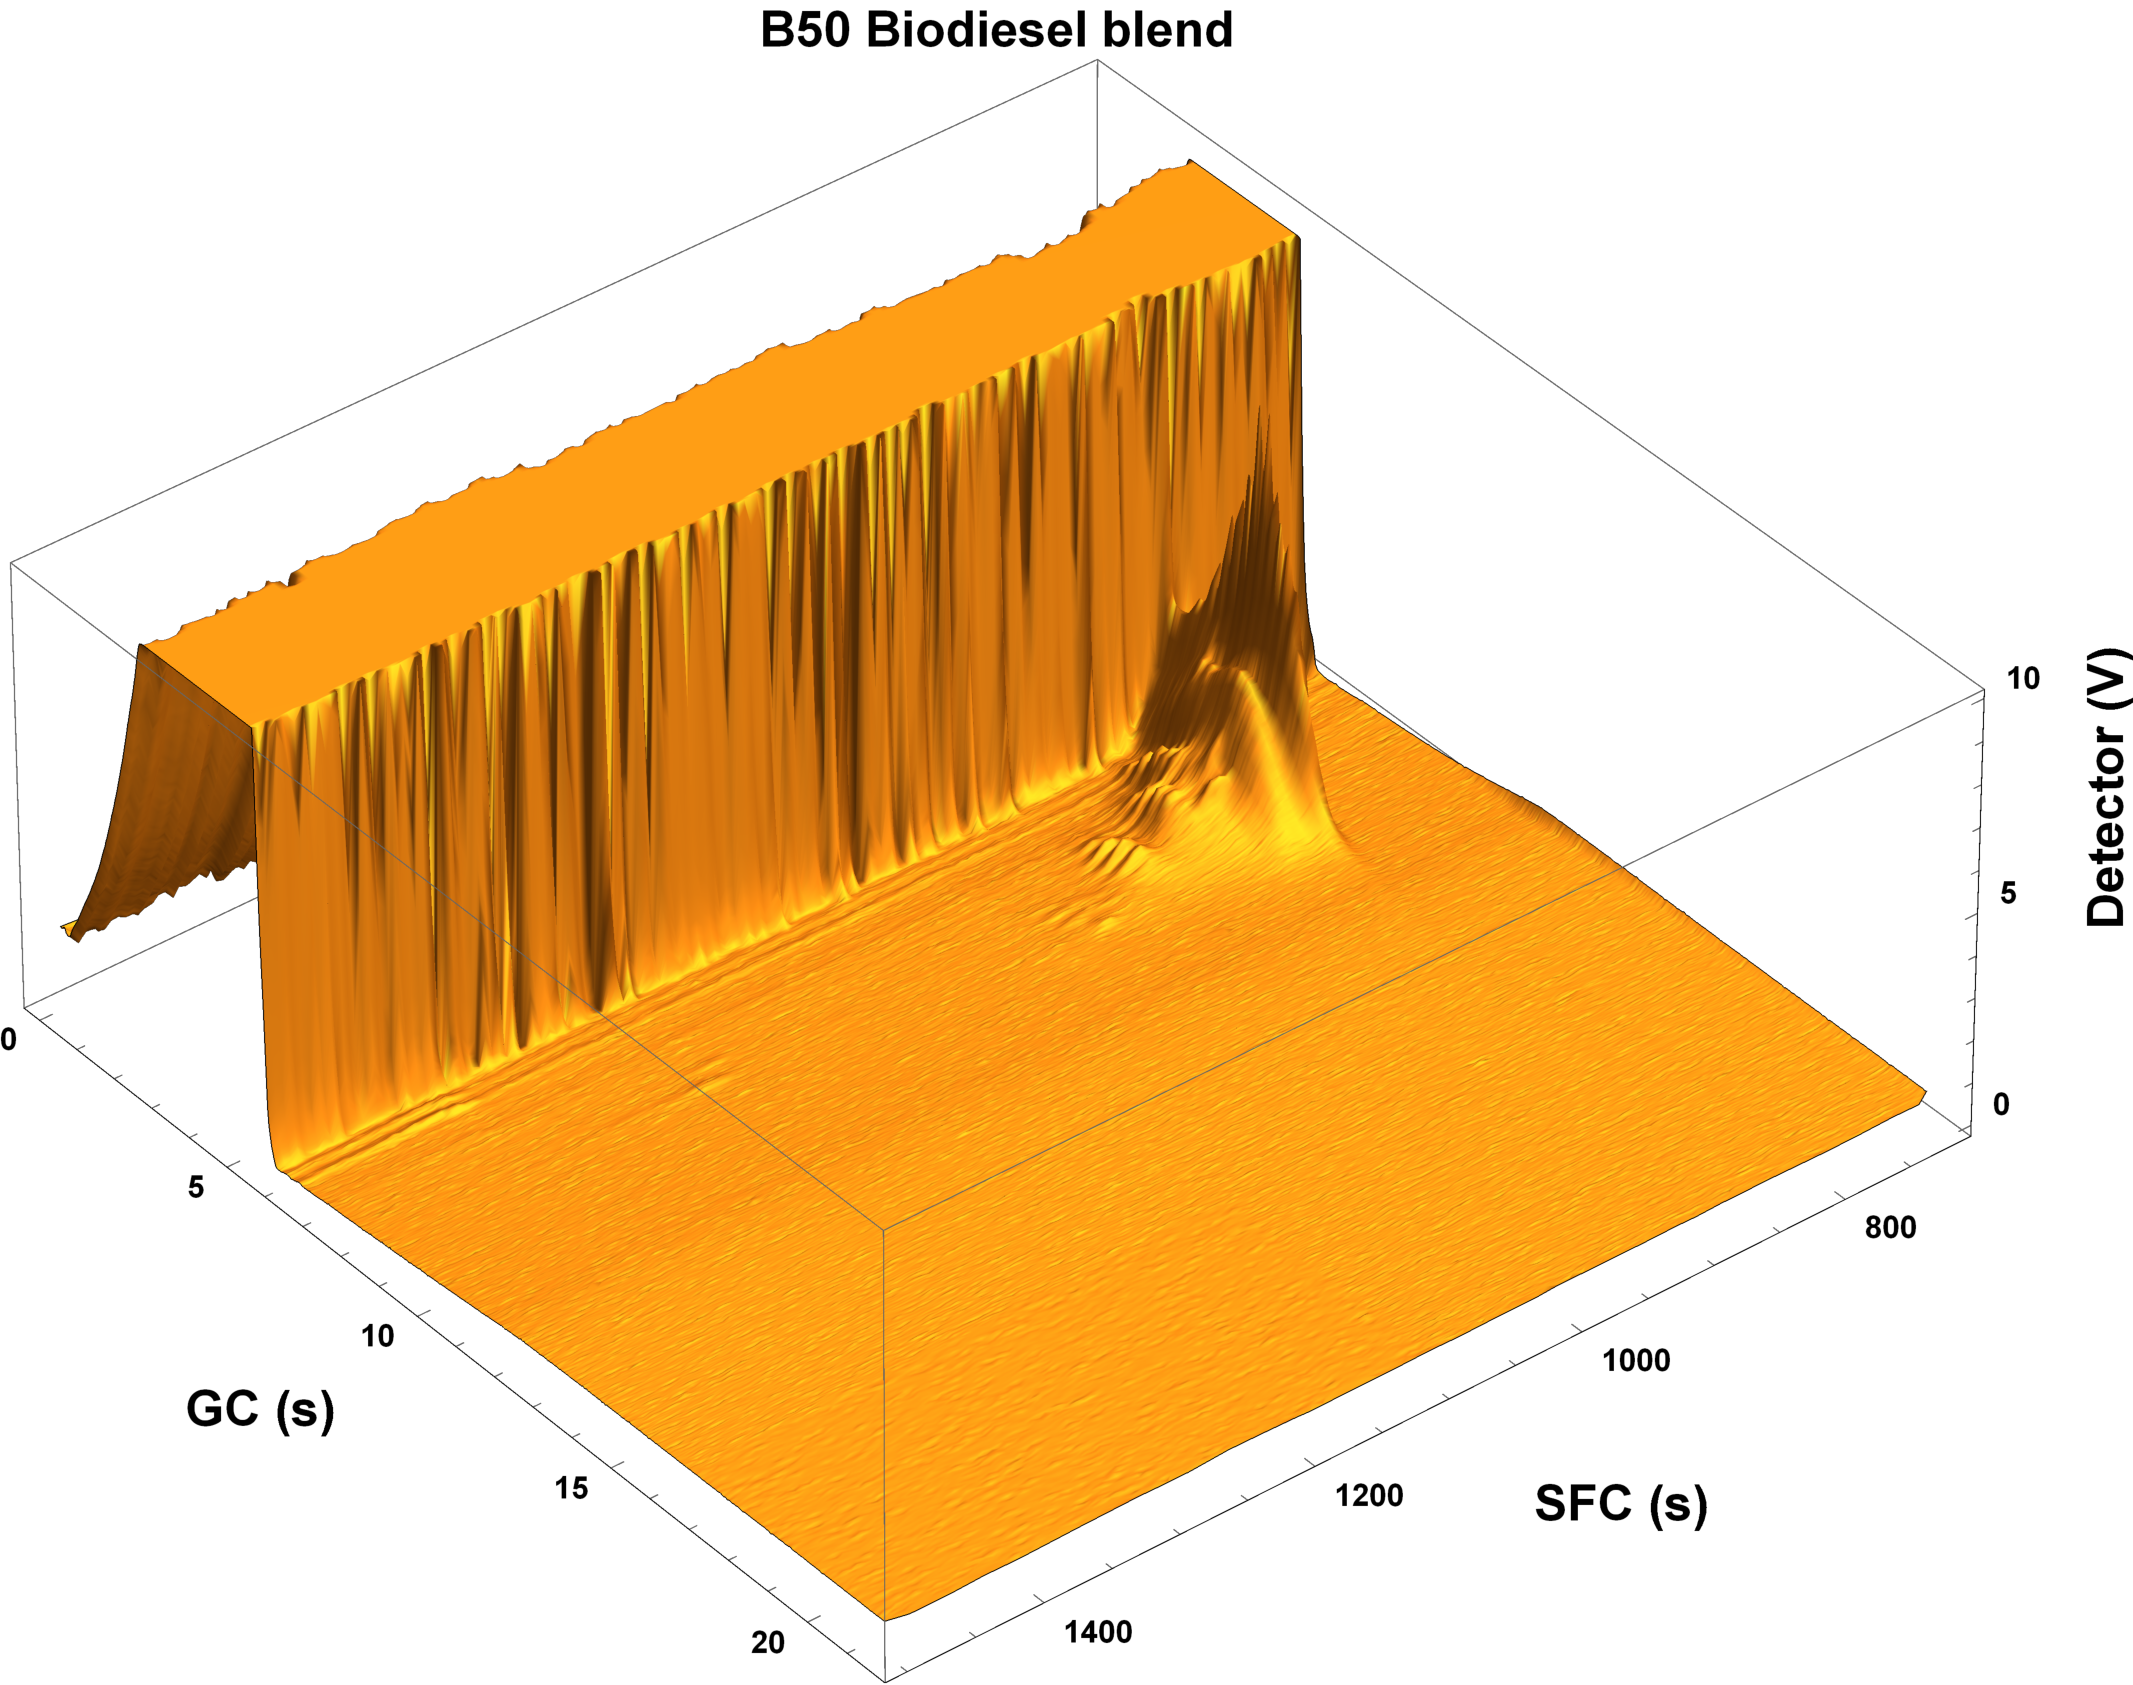
\includegraphics[width=0.8\textwidth]{Figures/Modifier.pdf}
	\decoRule	
	
	\caption[Modifiers in SFC]{The modifiers used in the SFC dimension elutes as a
solvent front on the GC dimension, and does not otherwise affect the separation.}
	
	\label{fig:Modifier} 
\end{figure}

\subsection{Discussion} 
% Chapter 8

\begin{savequote}[45mm]
In a book that I took from a shelf \ldots
\qauthor{Ancient proverb}
\end{savequote}

\chapter{Conclusion} % Main chapter title

\label{Chapter8} % For referencing this chapter elsewhere, use \ref{Chapter8}

%----------------------------------------------------------------------------------------
%	SECTION 1
%----------------------------------------------------------------------------------------

\section{Main Section 1}

%-----------------------------------
%	SUBSECTION 1
%-----------------------------------
\subsection{Subsection 1}

%-----------------------------------
%	SUBSECTION 2
%-----------------------------------

\subsection{Subsection 2}

%----------------------------------------------------------------------------------------
%	SECTION 2
%----------------------------------------------------------------------------------------

\section{Main Section 2}

%----------------------------------------------------------------------------------------
%	THESIS CONTENT - APPENDICES
%----------------------------------------------------------------------------------------

\appendix % Cue to tell LaTeX that the following "chapters" are Appendices

% Include the appendices of the thesis as separate files from the Appendices folder
% Uncomment the lines as you write the Appendices

%% Appendix A

\chapter{Index} % Main appendix title

\label{AppendixA} % For referencing this appendix elsewhere, use \ref{AppendixA}

% \printindex % The proper way

% The hack
\begin{theindex}
  
  \item \lowercase {acid rain}, \hyperpage{13}
  \item \lowercase {adopt}, \hyperpage{38}
  \item \lowercase {aerosol}, \hyperpage{2}
  \item \lowercase {auto-ignition temperature}, \hyperpage{10}
  \item \lowercase {autocatalytic}, \hyperpage{44}
  \item \lowercase {azeotropic mixture}, \hyperpage{18}
  \item \lowercase {back pressure regulator}, \hyperpage{62}
  \item \lowercase {biodiesel}, \hyperpage{19}
  \item \lowercase {biofuels}, \hyperpage{16}
  \item \lowercase {boiling point}, \hyperpage{28}
  \item \lowercase {caffeine}, \hyperpage{27}
  \item \lowercase {calibration}, \hyperpage{85}
  \item \lowercase {carbon footprint}, \hyperpage{6}
  \item \lowercase {carbon pollution}, \hyperpage{7}
  \item \lowercase {carbonated water}, \hyperpage{26}
  \item \lowercase {cetane number}, \hyperpage{42}
  \item \lowercase {chromatographic rate theory}, \hyperpage{69}
  \item \lowercase {chromatography}, \hyperpage{31}
  \item \lowercase {coal}, \hyperpage{1}
  \item \lowercase {coefficient of thermal expansion}, \hyperpage{100}
  \item \lowercase {cold filter plugging point}, \hyperpage{45}
  \item \lowercase {column bleed}, \hyperpage{100}
  \item \lowercase {combined cycle gas turbine}, \hyperpage{20}
  \item \lowercase {comprehensively coupled chromatography}, 
		\hyperpage{34}
  \item \lowercase {comprehensive}, \hyperpage{67}
  \item \lowercase {compression ratio}, \hyperpage{9}
  \item \lowercase {condenses}, \hyperpage{28}
  \item \lowercase {constraints}, \hyperpage{69}
  \item \lowercase {coulometric}, \hyperpage{47}
  \item \lowercase {criterion}, \hyperpage{69}
  \item \lowercase {critical point}, \hyperpage{29}
  \item \lowercase {crude oil}, \hyperpage{1}
  \item \lowercase {cryo-focusing}, \hyperpage{87}
  \item \lowercase {cryo-trapping}, \hyperpage{87}
  \item \lowercase {current}, \hyperpage{75}
  \item \lowercase {cut-off ratio}, \hyperpage{11}
  \item \lowercase {decaffeinated coffee}, \hyperpage{27}
  \item \lowercase {degree of unsaturation}, \hyperpage{47}
  \item \lowercase {derivatization reagent}, \hyperpage{50}
  \item \lowercase {detector overload}, \hyperpage{117}
  \item \lowercase {dielectric heating}, \hyperpage{75}
  \item \lowercase {dip tube}, \hyperpage{89}
  \item \lowercase {discrimination}, \hyperpage{62}
  \item \lowercase {drying oil}, \hyperpage{109}
  \item \lowercase {efficiency optimized velocity}, \hyperpage{70}
  \item \lowercase {efficiency-optimized flow}, \hyperpage{70}
  \item \lowercase {efficiency}, \hyperpage{7}, \hyperpage{70}
  \item \lowercase {electrometer}, \hyperpage{32}
  \item \lowercase {electron capture detector}, \hyperpage{71}
  \item \lowercase {emissivity}, \hyperpage{78, 79}
  \item \lowercase {error}, \hyperpage{57}
  \item \lowercase {exhaust gas recirculation}, \hyperpage{14}
  \item \lowercase {fast chromatography}, \hyperpage{68}
  \item \lowercase {fast}, \hyperpage{35}, \hyperpage{122}
  \item \lowercase {first dimension}, \hyperpage{34}
  \item \lowercase {flame ionization detector}, \hyperpage{32}
  \item \lowercase {flash point}, \hyperpage{43}
  \item \lowercase {fly ash}, \hyperpage{2}
  \item \lowercase {four wire resistance measurement}, \hyperpage{125}
  \item \lowercase {fracture toughness}, \hyperpage{98}
  \item \lowercase {front}, \hyperpage{116}
  \item \lowercase {fuel cell}, \hyperpage{15}
  \item \lowercase {gas chromatography}, \hyperpage{31}
  \item \lowercase {gas turbine}, \hyperpage{11}
  \item \lowercase {general elution problem}, \hyperpage{72}
  \item \lowercase {goal}, \hyperpage{68}
  \item \lowercase {gradient elution}, \hyperpage{72}
  \item \lowercase {green chemistry}, \hyperpage{18}, \hyperpage{25}
  \item \lowercase {heart-cutting}, \hyperpage{34}
  \item \lowercase {high performance liquid chromatography}, 
		\hyperpage{31}
  \item \lowercase {holds}, \hyperpage{73}
  \item \lowercase {hydrogen}, \hyperpage{16}
  \item \lowercase {ignition delay}, \hyperpage{43}
  \item \lowercase {induction period}, \hyperpage{44}
  \item \lowercase {inductive heating}, \hyperpage{75}
  \item \lowercase {injector}, \hyperpage{42}
  \item \lowercase {input power}, \hyperpage{7}
  \item \lowercase {internal\hyp  {}combustion engines}, \hyperpage{6}
  \item \lowercase {iodine value}, \hyperpage{47}
  \item \lowercase {isolation amplifier}, \hyperpage{124}
  \item \lowercase {kinetic optimization}, \hyperpage{69}
  \item \lowercase {knocking}, \hyperpage{11}
  \item \lowercase {lean-burn}, \hyperpage{14}
  \item \lowercase {life cycle analysis}, \hyperpage{6}
  \item \lowercase {linear power supply}, \hyperpage{125}
  \item \lowercase {linseed oil}, \hyperpage{107}
  \item \lowercase {liquid chromatography}, \hyperpage{31}
  \item \lowercase {lubricity}, \hyperpage{53}
  \item \lowercase {manipulated variable}, \hyperpage{57}
  \item \lowercase {modifier}, \hyperpage{30}
  \item \lowercase {modulation period}, \hyperpage{68}
  \item \lowercase {modulation rate}, \hyperpage{68}
  \item \lowercase {modulators}, \hyperpage{67}
  \item \lowercase {natural gas}, \hyperpage{1}
  \item \lowercase {noxious pollution}, \hyperpage{7}
  \item \lowercase {number of plates}, \hyperpage{60}, \hyperpage{70}
  \item \lowercase {ocean acidification}, \hyperpage{4}
  \item \lowercase {octane number}, \hyperpage{11}
  \item \lowercase {optimization}, \hyperpage{68}
  \item \lowercase {optimizing parameters}, \hyperpage{69}
  \item \lowercase {orthogonal}, \hyperpage{34}
  \item \lowercase {output power}, \hyperpage{7}
  \item \lowercase {overload}, \hyperpage{116}
  \item \lowercase {ozone}, \hyperpage{12}
  \item \lowercase {payload}, \hyperpage{15}
  \item \lowercase {peak resolution}, \hyperpage{60}
  \item \lowercase {peak tailing}, \hyperpage{60}
  \item \lowercase {peak width}, \hyperpage{70}
  \item \lowercase {petrodiesel}, \hyperpage{38}, \hyperpage{109}
  \item \lowercase {photochemical smog}, \hyperpage{13}
  \item \lowercase {photovoltaic}, \hyperpage{16}
  \item \lowercase {plate height}, \hyperpage{70} 
  \item \lowercase {pollution}, \hyperpage{2}
  \item \lowercase {polycyclic aromatic hydrocarbons}, \hyperpage{51}
  \item \lowercase {polyimide resin}, \hyperpage{98}
  \item \lowercase {porous layer open tubular}, \hyperpage{51}
  \item \lowercase {power}, \hyperpage{75}
  \item \lowercase {process variable}, \hyperpage{57}
  \item \lowercase {property}, \hyperpage{40}
  \item \lowercase {pulse width modulation control}, \hyperpage{125}
  \item \lowercase {pulse width modulation}, \hyperpage{87}
  \item \lowercase {pyro-synthesis}, \hyperpage{12}
  \item \lowercase {radiative heating}, \hyperpage{75}
  \item \lowercase {ramp rate}, \hyperpage{73}
  \item \lowercase {ramps}, \hyperpage{73}
  \item \lowercase {rancid}, \hyperpage{44}
  \item \lowercase {real-time operating systems.}, \hyperpage{126}
  \item \lowercase {requirement}, \hyperpage{40}
  \item \lowercase {resistance}, \hyperpage{75}
  \item \lowercase {resistive heating}, \hyperpage{75}
  \item \lowercase {restrictor}, \hyperpage{62}
  \item \lowercase {retention factor}, \hyperpage{60}, \hyperpage{72}
  \item \lowercase {retention times}, \hyperpage{57}
  \item \lowercase {retention time}, \hyperpage{70}
  \item \lowercase {retention volumes}, \hyperpage{57}
  \item \lowercase {run time}, \hyperpage{68}
  \item \lowercase {sample cleanup}, \hyperpage{71}
  \item \lowercase {sample throughput}, \hyperpage{68}
  \item \lowercase {second dimension}, \hyperpage{34}
  \item {Seebeck effect}, \hyperpage{81}
  \item \lowercase {selective detection}, \hyperpage{71}
  \item \lowercase {selective}, \hyperpage{28}
  \item \lowercase {selectivity}, \hyperpage{60}
  \item \lowercase {selectivity optimization}, \hyperpage{69}
  \item \lowercase {separation}, \hyperpage{31}
  \item \lowercase {set value}, \hyperpage{57}
  \item \lowercase {silicon mica}, \hyperpage{89}
  \item \lowercase {single ion monitoring}, \hyperpage{72}
  \item \lowercase {soaps}, \hyperpage{48}
  \item \lowercase {solar methanol}, \hyperpage{16}
  \item \lowercase {solid phase extraction}, \hyperpage{72}
  \item \lowercase {speed-optimized flow}, \hyperpage{71}
  \item \lowercase {standards organizations}, \hyperpage{38}
  \item \lowercase {standard}, \hyperpage{37}
  \item \lowercase {storage battery}, \hyperpage{15}
  \item \lowercase {stratified charge}, \hyperpage{14}
  \item \lowercase {supercritical fluid chromatography}, \hyperpage{31}
  \item \lowercase {supercritical fluid extraction}, \hyperpage{28}
  \item \lowercase {switched-mode power supply}, \hyperpage{125}
  \item \lowercase {technical committees}, \hyperpage{38}
  \item \lowercase {technical standards}, \hyperpage{37}
  \item \lowercase {temperature programming}, \hyperpage{72}
  \item \lowercase {tensile strength}, \hyperpage{98}
  \item \lowercase {test method}, \hyperpage{40}
  \item \lowercase {thermal fatigue}, \hyperpage{101}
  \item \lowercase {thermal imaging}, \hyperpage{78}
  \item \lowercase {thermal shock}, \hyperpage{100}
  \item \lowercase {thermocouple}, \hyperpage{81}
  \item \lowercase {thin-film case}, \hyperpage{70}
  \item \lowercase {thin-layer chromatography}, \hyperpage{34}
  \item \lowercase {total contamination}, \hyperpage{46}
  \item \lowercase {transesterification}, \hyperpage{19}
  \item \lowercase {triple point}, \hyperpage{29}
  \item \lowercase {tunable}, \hyperpage{28}
  \item \lowercase {tuning}, \hyperpage{90}
  \item  {van Deemter equation}, \hyperpage{70}
  \item \lowercase {virtual instruments}, \hyperpage{92}
  \item \lowercase {visual programming language}, \hyperpage{92}
  \item \lowercase {void time}, \hyperpage{70}
  \item \lowercase {voltage}, \hyperpage{75}
  \item \lowercase {wear scar}, \hyperpage{53}
  \item \lowercase {wrap-around}, \hyperpage{73}

\end{theindex}

% Appendix Template

\chapter{Glossary} % Main appendix title

\label{AppendixB} % Change X to a consecutive letter; for referencing this appendix elsewhere, use \ref{AppendixX}

A list of technical terms that might be unfamiliar to the reader. 

\begin{description}
	\item[Azeotropic mixture]A mixture of liquids in which the vapour phase and the liquid phase have the same composition. The mixture cannot be further purified by simple distillation.
	\item[Payload]The portion of the weight of a vehicle's load that is in excess of what it needs to complete a journey. This 

\end{description}

%% Appendix Template

\chapter{Thermocouple Production} % Main appendix title

\label{AppendixC} % Change X to a consecutive letter; for referencing this appendix elsewhere, use \ref{AppendixX}

How the thermocouple probe was made:

\begin{enumerate}
  \item 
	\item A piece of 0.25 mm polyimide-coated fused-silica capillary of about 500 mm length was cut and mounted with sticky tape on a wooden metre stick.
	\item A longer length of 0.1 mm fused-silica capillary was threaded through the 0.25 mm capillary.
	\item The end of one of the thermocouple wires was inserted into the end of the 0.1 mm capillary. A drop of cyanoacrylate adhesive was touched to the end of the capillary. Capillary action drew the liquid adhesive into the capillary and fixed the wire in place.
	\item The wire was drawn carefully into the capillary by pulling on the 0.1 mm capillary.
	\item Once the end of the wire protruded through the end of the 0.25 mm capillary the end of the 0.1 mm capillary was cut off.
	\item The wire was anchored at one end with adhesive tape, pulled tight, and anchored at the other end. 
	\item The procedure was repeated for the other wire.
	\item The two thermocouple wires (Goodfellow) was clamped in a twisting bar. The twister bar has a square profile, 8 mm on a side.
	\item The wires were flamed with a cigar lighter until they were red a dull red hot. (At any higher temperature the wires would melt.) This chars the polyimide coating.
	\item The flamed portion of the wires were lightly sanded with 1200 grit water paper. A pair of small pliers had its beak lined with the abrasive, and lightly stroked up and down the wire to remove the char.
	\item A 6 mm tube was inserted between the wires to serve as spacer. and moved until about 10mm away from the twister bar.
	\item The wires were twisted by turning the twister bar until the twister portion was about 5mm long.
	\item The spools were rewound to retract the wire, until the start of the twist rested on the clamping bar.
	\item The clamping weight was lowered onto the clamping bar, keeping the pair or wires in place.
	\item A small pair of scissors was used to snip off the end of the
	\item The welding electrode was brought into position. This was a carbon rod in the form of a pencil lead (Schwann Stabilo), 2 mm in diameter, mounted on a screwing connector. The welding circuit consisted of a bench power supply set to approximately 20V. connected. The negative terminal was clamped to the aluminium base plate of the microscope, on which rested the brass clamp bar. The positive terminal was clamped to the carbon electrode. A voltage of approximately 23 V was applied.
	\item It was discovered that the carbon electrode should not have a polished end, but a roughly broken end. 
	\item The electrode was moved closer to the clamped twisted wire.
	\item At the right point a spark would jump from the carbon to the wire, melting the end of the wire. The molten wire would draw into a globule on the end of the wire, withdrawing from the electrode and so breaking the spark, ending the heating.
	\item If the wire would actually touch the electrode the wire would heat up red hot and melt off, usually destroying the twist and requiring making a new twist.
	\item If all went well, there would be a hemispherical weld at the end of the twist where the two wires would be joined.
	\item The thermocouple wires was withdrawn into the capillary until the end just protruded, kept in place with a pair of rubber-tipped self-closing tweezers.
	\item If two sets of thermocouples were needed, the procedure would be repeated for another pair of wires.
	\item The wires would be pulled back, one pair at a time.
	\item The other end of the capillary was taped to the connector pad.
	\item The wires was flamed and scraped to remove the polyimide isolation, and screwed down on a screw connector block.
	\item The resistance between the protruding end of the thermocouple and the connector block was measured to ensure electrical connection. The resistance for the Chromel is 1440 $\Omega{m}^{-1}$, and for the Alumel 600 $\Omega{m}^{-1}$
	\item A drop of cyanoacrylate adhesive was put on the end of the capillary to anchor the wires and to prevent high-pressure gas from blowing the wires out of the capillary. 
\end{enumerate}

% Appendix Template

\chapter{Engineering Drawings} % Main appendix title

\label{AppendixD} 


% Appendix E

\chapter{Fatty acid profiles} % Main appendix title

\label{AppendixE} % Change X to a consecutive letter; for referencing this appendix elsewhere, use \ref{AppendixX}

\begin{table}
\centering
\caption{The fatty acid profile of sunflower oil sample}
\label{tab:SunflowerPrecisionOils}
\begin{tabular}{c|c}
\toprule
\tabhead{Fatty acid} & \tabhead{Fraction}\\
\midrule
C14:0 & 0.05 \\ \hline
C16:0 & 6.14 \\ \hline
C16:1 & 0.04 \\ \hline
C17:0 & 0.05 \\ \hline
C17:1 & 0 \\ \hline
C18:0 & 5.77 \\ \hline
C18:1 t & 0 \\ \hline
C18:1 c & 21.21 \\ \hline
C18:2 t & 0 \\ \hline
C18:2 c & 63.91 \\ \hline
C18:3n6 & 0.11 \\ \hline
C18:3n3 & 1.04 \\ \hline
C20:0 & 0.47 \\ \hline
C20:1 & 0.24 \\ \hline
C20:2 & 0 \\ \hline
C21:0 & 0 \\ \hline
C22:0 & 0.77 \\ \hline
C22:1 & 0 \\ \hline
C24:0 & 0.19 \\ \hline
C24:1 & 0 \\ \hline
\bottomrule\\
\end{tabular}
\end{table}

\begin{table}
	\caption{Fatty acid profile of coconut oil according to the FAO \autocite{JFAOWHOCAC2019}}
	\label{tab:CoconutFAO}
	\centering
\begin{tabular}{c|c|c}
\toprule
	\tabhead{Fatty acid} & \tabhead{Lower} &   	\autocite{Upper}	\\
	\midrule
C6:0	&ND&	0.7	\\
C8:0	&4.6	&10\\
C10:0	&5	&8	\\
C12:0	&45.1	&53.2	\\
C14:0	&16.8	&21	\\
C16:0	&7.5	&10.2	\\
C16:1	&ND	&	\\
C17:0	&ND	&	\\
C17:1	&ND	&	\\
C18:0	&2	&4	\\
C18:1	&5	&10	\\
C18:2	&1	&2.5	\\
C18:3	&ND	&0.2	\\
C20:0	&ND	&0.2	\\
C20:1	&ND	&0.2	\\
C20:2	&ND	&	\\
C22:0	&ND	&	\\
C22:1	&ND	&	\\
C22:2	&ND	&	\\
C24:0	&ND	&	\\
C24:1	&ND	&	\\
	\bottomrule\\
\end{tabular}
\end{table}



%----------------------------------------------------------------------------------------
%	BIBLIOGRAPHY
%----------------------------------------------------------------------------------------

\printbibliography[heading=bibintoc]

%----------------------------------------------------------------------------------------

\end{document}  
